\documentclass[12pt]{amsart}

% %%%%%%%%%%%%%%%%%%%%%%%%%%%%%%%%%%%%%%%%%%%%%%%%%%%%%%%%%%%
% FONT ENCODING

\usepackage[T1]{fontenc}
\usepackage[utf8]{inputenc}
\usepackage{lmodern}

% %%%%%%%%%%%%%%%%%%%%%%%%%%%%%%%%%%%%%%%%%%%%%%%%%%%%%%%%%%%
% PACKAGES

% Math packages
\usepackage{amsmath,amsthm,amsfonts,amssymb,mathtools}

% fonts
\usepackage[mathscr]{eucal} % script
\usepackage{bbm} % lower case mathbb

% for upright Greek letters
\usepackage{upgreek}

% graphics
\usepackage{graphicx}

% tables
\usepackage{booktabs}

% diagrams and figures
\usepackage{tikz}
% \usetikzlibrary{quantikz}  % quantum gates!
\usetikzlibrary{quantikz2}
\usetikzlibrary{cd}  % commutative diagrams
\usetikzlibrary{angles}

% references
\usepackage{varioref}

% better lists
\usepackage[shortlabels]{enumitem}
% \setlist[enumerate]{itemsep=1.3ex}
% \setlist[itemize]{itemsep=1.3ex}

% quantum computing
\usepackage{braket}

% index
\usepackage{imakeidx}
\makeindex
\makeindex[name=not,title=Notation]
% %%%%%%%%%%%%%%%%%%%%%%%%%%%%%%%%%%%%%%%%%%%%%%%%%%%%%%%%%%%
% FORMATTING

% page
\usepackage[textwidth=6in,textheight=8.5in]{geometry}

% paragraph indent
\setlength{\parindent}{0pt}

% space between paragraphs
\setlength{\parskip}{1cm plus4mm minus3mm} % default 1cm with + 4mm or
% -3mm adjustments
% interline space
\usepackage{setspace}
\setstretch{1.33}

\usepackage{hyperref}  % hyperlinks
\usepackage[poorman,capitalize]{cleveref}

% %%%%%%%%%%%%%%%%%%%%%%%%%%%%%%%%%%%%%%%%%%%%%%%%%%%%%%%%%%%
% THEOREM STYLING

% theorems

\theoremstyle{plain}
\newtheorem{theorem}{Theorem}[section]
\newtheorem{proposition}[theorem]{Proposition}
\newtheorem{corollary}[theorem]{Corollary}
\newtheorem{lemma}[theorem]{Lemma}
\newtheorem{conjecture}[theorem]{Conjecture}

\theoremstyle{definition}
\newtheorem{definition}[theorem]{Definition}
\newtheorem{notation}[theorem]{Notation}

\theoremstyle{remark}
\newtheorem*{remark}{Remark}
\newtheorem*{remarks}{Remarks}
\newtheorem{example}[theorem]{Example}
\newtheorem*{ack}{Acknowledgments}


% %%%%%%%%%%%%%%%%%%%%%%%%%%%%%%%%%%%%%%%%%%%%%%%%%%%%%%%%%%%
% FONTS AND SHORTCUTS


% fonts shortcuts
\newcommand{\ecal}{\mathscr}
\newcommand{\mcal}{\mathcal}


% Sets
\newcommand{\F}{\mathbb{F}}
\newcommand{\R}{\mathbb{R}}
\newcommand{\N}{\mathbb{N}}
\newcommand{\Z}{\mathbb{Z}}
\newcommand{\Q}{\mathbb{Q}}
\newcommand{\C}{\mathbb{C}}

% e, i, and pi
\newcommand{\me}{\mathrm{e}}
\newcommand{\mi}{\mathrm{i}}
\newcommand{\mpi}{\uppi}
\newcommand{\md}{\mathrm{d}} % for derivatives

% shortcuts
\newcommand{\idef}{\overset{{\rm def}}{=}}
\newcommand{\abs}[1]{\left| #1 \right|}
\newcommand{\floor}[1]{\left\lfloor{#1}\right\rfloor}
\newcommand{\ceil}[1]{\left\lceil{#1}\right\rceil}

% such that
\newcommand{\st}{\;{:}\;}

% replace bar with overline
\renewcommand{\bar}{\overline}

% some operators
\DeclareMathOperator{\lcm}{lcm}
\DeclareMathOperator{\GL}{GL}
\DeclareMathOperator{\SL}{SL}
\DeclareMathOperator{\ord}{ord}
\DeclareMathOperator{\chr}{char} % characteristic

% %%%%%%%%%%%%%%%%%%%%%%%%%%%%%%%%%%%%%%%%%%%%%%%%%%%%%%%%%%%
% EXTRA SHORTCUTS

\newcommand{\cnot}{\mathrm{CNOT}}  % CNOT gate
\newcommand{\adj}[1]{#1^{\dagger}}  % adjoint
\DeclareMathOperator{\U}{U}  % unitary matrices
\newcommand{\un}{\U_n(\C)}
\newcommand{\idt}{\mathbb{I}}
\newcommand{\prob}{\mathbb{P}}
\newcommand{\ft}{\mathcal{F}}  % Fourier transform
\DeclareMathOperator{\qft}{QFT}  % quantum Fourier transform
\DeclareMathOperator{\qpe}{QPE}  % quantum phase estimator
\DeclareMathOperator{\mmod}{mod}
\DeclareMathOperator{\swpg}{SWAP}
\DeclareMathOperator{\cswp}{CSWAP}
\DeclareMathOperator{\spec}{spec}
\DeclareMathOperator{\Poly}{Poly}
\DeclareMathOperator{\sspan}{span}
\DeclareMathOperator{\stab}{stab}
\newcommand{\shr}[1]{#1^{\mathrm{Shor}}}

% %%%%%%%%%%%%%%%%%%%%%%%%%%%%%%%%%%%%%%%%%%%%%%%%%%%%%%%%%%%


\title{Notes on Quantum Computing}
\author{Luís R.~A.~Finotti}


% %%%%%%%%%%%%%%%%%%%%%%%%%%%%%%%%%%%%%%%%%%%%%%%%%%%%%%%%%%%
% DOCUMENT

\begin{document}

\maketitle

\tableofcontents

\section{Qubits}

\begin{notation}
  The following notation is commonly used:

  \begin{enumerate}[itemsep=2ex]

  \item{} \emph{Qubit}\index{qubit}:
    \begin{align*}
      % \ket{0}\index[not]{ket zero@$\ket{0}$} &\idef \begin{pmatrix}
      %   1 \\
      %   0
      % \end{pmatrix},
      % & \ket{1}\index[not]{ket one@$\ket{1}$} &\idef \begin{pmatrix}
      %   0 \\
      %   1
      % \end{pmatrix} \\
      % \ket{+}\index[not]{ket plus@$\ket{+}$} &\idef \begin{pmatrix}
      %   \sqrt{2}/2 \\
      %   \sqrt{2}/2
      % \end{pmatrix},
      % & \ket{-}\index[not]{ket minus@$\ket{-}$} &\idef \begin{pmatrix}
      %   \sqrt{2}/2 \\
      %   -\sqrt{2}/2
      % \end{pmatrix} \\
      % \ket{\mi}\index[not]{ket i@$\ket{\mi}$} &\idef \begin{pmatrix}
      %   \sqrt{2}/2 \\
      %   \sqrt{2}/2 \mi
      % \end{pmatrix},
      % & \ket{-\mi}\index[not]{ket minus i@$\ket{-\mi}$} &\idef \begin{pmatrix}
      %   \sqrt{2}/2 \\
      %   -\sqrt{2
      %   }/2 \mi
      %  \end{pmatrix}
    \end{align*}

    \[
      \ket{0}\index[not]{ket zero@$\ket{0}$} \idef \begin{pmatrix}
        1 \\
        0
      \end{pmatrix}, \qquad
       \ket{1}\index[not]{ket one@$\ket{1}$} \idef \begin{pmatrix}
        0 \\
        1
      \end{pmatrix},
    \]
    \[
      \ket{+}\index[not]{ket plus@$\ket{+}$} \idef \frac{\sqrt{2}}{2} \begin{pmatrix}
        1 \\
        1
      \end{pmatrix} , \qquad
       \ket{-}\index[not]{ket minus@$\ket{-}$} \idef \frac{\sqrt{2}}{2} \begin{pmatrix}
         1 \\
         -1
       \end{pmatrix}
    \]
    \[
      \ket{\mi}\index[not]{ket i@$\ket{\mi}$} \idef \frac{\sqrt{2}}{2}  \begin{pmatrix}
        1 \\
        \mi
      \end{pmatrix} , \qquad
       \ket{-\mi}\index[not]{ket minus i@$\ket{-\mi}$} \idef \frac{\sqrt{2}}{2} \begin{pmatrix}
         1 \\
         -\mi
       \end{pmatrix}.
    \]

\item{} \emph{Quantum State}\index{quantum state}:
  \[
    \ket{\psi}\index[not]{ket psi@$\ket{\psi}$} = \begin{pmatrix}
      \alpha \\
      \beta
    \end{pmatrix} , \qquad \text{with } |\alpha|^2 + |\beta|^2 = 1,
  \]
  where $|\alpha|^2$ is the probability of the qubit measuring as the $0$ state and $|\beta|^2$ is the probability of the qubit measuring as the $1$ state.

\item{} \emph{Dirac Notation}\index{Dirac notation} (and the \emph{ket vector}\index{ket vector}):
  \[
    \ket{\psi} = \begin{pmatrix}
      \alpha \\
      \beta
    \end{pmatrix} = \alpha \ket{0} + \beta \ket{1}.
  \]

\item We denote by $\oplus$ the addition in $\F_2$.  E.g., if $x \in \F_2$, we have that
  \[
    \ket{x \oplus 1} =
    \begin{cases}
      1, & \text{if $x = 0$};\\
      0, & \text{if $x = 1$}.
    \end{cases}
  \]
  (So, this is example is like the \emph{not} gate.)

\item
  \[
     \ket{\psi(\theta, \phi)}\index[not]{ket theta phi@$\ket{\psi(\theta, \phi)}$} \idef \cos(\theta/2) \ket{0} + \me^{\mi \phi} \sin(\theta/2) \ket{1}.
  \]
  (See \cref{sec:bloch_sphere} below.)

\item If $\ket{\phi} = \lambda \ket{\psi}$ with $\abs{\lambda} = 1$, then $\ket{\phi}$ and $\ket{\psi}$ are \emph{physically equivalent}.  So we can disregard the overall phase.

\end{enumerate}
\end{notation}


\section{Tensor Products}\label{sec:tensor_prods}


\begin{notation}
  We denote, e.g.,
  \[
    \ket{010011} \idef \ket{0} \otimes \ket{1} \otimes \ket{0} \otimes \ket{0} \otimes \ket{1} \otimes \ket{1}.
  \]
  Also, as usual,
  \[
    \ket{0}^{\otimes 5} \idef \ket{00000}.
  \]
\end{notation}

\begin{remark}
  If we have $\alpha \ket{00} + \beta \ket{01} + \gamma \ket{10} + \delta \ket{11}$, then
  \begin{align*}
    |\alpha|^2 &= \text{probability of measuring $\ket{00}$}, \\
    |\beta|^2 &= \text{probability of measuring $\ket{01}$}, \\
    |\gamma|^2 &= \text{probability of measuring $\ket{10}$}, \\
    |\delta|^2 &= \text{probability of measuring $\ket{11}$}.
  \end{align*}
\end{remark}



\begin{definition}
  The \emph{computational basis}\index{computational basis} is simply the induced basis of ${\left({\C^2}\right)}^{\otimes n}$: $\{\ket{i_1i_2 \ldots i_n} \st i_j \in \{0, 1\}\}$.  The order in qiskit is done via the binary representation (with unit digit coming \emph{first}), e.g.,
  \[
    \{\ket{000}, \ket{100}, \ket{010}, \ket{110}, \ket{001}, \ket{101}, \ket{011}, \ket{111}\}.
  \]
  One can sometimes represent this basis (in this same order) as
  \[
    \{\ket{0}_3, \ket{1}_3, \ket{2}_3, \ket{3}_3, \ldots, \ket{7}_3\}.
  \]
\end{definition}



\section{Inner Product}

We have the \emph{inner product}\index{inner product} in ${\left( {\C^2} \right)}^{\otimes n}$:  if $\ket{\psi}  = \sum_{x \in \F_2^n} \psi_x \ket{x}$ and $\ket{\phi} = \sum_{x \in \F_2^n} \phi_x \ket{x}$, then
\[
  \langle \psi \mid \phi  \rangle \idef \sum_{x \in \F_2^n} \bar{\psi}_x \phi_x.
\]
(So, it is simply the inner product that makes the computational basis \emph{orthonormal}.)

Of course, for $x, y \in \F_2^n$, we have that $\langle x \mid y  \rangle = \delta_{x, y}$.

Note that we denote by $\bra{\psi}\index[not]{bar psi@$\bra{\psi}$}$ (the \emph{bra vector}\index{bra vector} of $\psi$) the dual element of $\ket{\psi}$:
\[
  \bra{\psi} = \sum_{x \in \F_2^n} \bar{\psi}_x \bra{x}.
\]
Hence,
\[
  \bra{\psi} \ket{\phi} = \langle \psi \mid \phi  \rangle.
\]




\section{Bloch Sphere}\label{sec:bloch_sphere}

\textbf{Reference:} \href{https://www.youtube.com/watch?v=AYGHS9hXgyw}{Bloch Sphere | Visualizing Qubits and Spin | Quantum Information}


Note that if $|\rho|=1$, then $\ket{\psi} \sim \rho \ket{\psi}$, as we don't care about the \emph{overall} phase.  So, if
\[
  \ket{\psi} = \begin{pmatrix}
    \alpha \\
    \beta
  \end{pmatrix} = \alpha \ket{0} + \beta \ket{1},
\]
then $|\alpha|^2 + |\beta|^2 = 1$, so
\begin{align*}
  \alpha &= \cos(\gamma) \me^{\mi \delta}, \\
  \beta &= \sin(\gamma) \me^{\mi \epsilon},
\end{align*}
with $\gamma, \delta, \epsilon \in \R$.  Now,
\begin{align*}
  \ket{\psi} &= \cos(\gamma) \me^{\mi \delta} \ket{0} + \sin(\gamma) \me^{\mi \epsilon} \ket{1} \\
             &=\me^{\mi \delta} \left( \cos(\gamma) \ket{0} + \me^{\mi (\epsilon - \delta)} \sin(\gamma) \ket{1}\right) \\
  &\sim \cos(\gamma) \ket{0} + \me^{\mi (\epsilon - \delta)} \sin(\gamma) \ket{1}.
\end{align*}


So, we have that
\begin{equation}\label{eq:bloch_coord}
  \ket{\psi} \sim \ket{\psi(\theta, \phi)} \idef \cos(\theta/2) \ket{0} + \me^{\mi \phi} \sin(\theta/2) \ket{1}, \qquad \theta \in [0, \mpi], \; \phi \in [0, 2 \mpi].
\end{equation}

Note that $\epsilon - \delta$ is the \emph{relative phase}\index{relative phase}.  Clearly, the relative phase does not change the probabilities.

Considering:
\begin{itemize}

\item $\theta$ the angle in $\R^3$ with the $z$-axis;

\item $\phi$ the angle in $\R^3$ with the $x$-axis around the $z$-axis;

\end{itemize}
we get a sphere (with spherical coordinates and radius $1$), the \emph{Bloch sphere}\index{Bloch sphere} (in \vref{fig:bloch_sphere}).

\begin{figure}\centering

  \includegraphics[scale=0.15]{Bloch_sphere.png}

  \caption{Bloch Sphere}\label{fig:bloch_sphere}
\end{figure}

Let
\[
  \hat{\eta} = \begin{pmatrix}
    \sin(\theta)\cos(\phi) \\
    \sin(\theta)\sin(\phi) \\
    \cos(\theta)
  \end{pmatrix}
\]
be a direction/point on the sphere (in spherical coordinates).  Then, the spin operator in the direction of $\hat{\eta}$ (with angles $\theta$ and $\phi$ as above) the Bloch state $\ket{\psi(\theta, \phi)}$ is an eigenfunction with positive eigenvalue $\hbar/2$.  (FIXME!  Need details!)


\section{Gates}

\begin{definition}
  A $1$-qubit \emph{gate}\index{gate} is simply an element of $\U_2(\C)$ acting on a singe qubit.  More gerenerally an $n$-qubit gate is an element of $U_{2^n}(\C)$.
\end{definition}

\begin{notation}
  \begin{enumerate}

  \item{} \emph{$X$ Gate\index{X gate@$X$ gate}}: multiplication by:
    \[
      X\index[not]{X@$X$} \idef \left(
        \begin{array}{rr}
          0 & 1 \\
          1 & 0
        \end{array}\right)
    \]
    It is basically the NOT gate, $\ket{x} \mapsto \ket{x \oplus 1}$.  So, $\alpha \ket{0} + \beta \ket{1} \mapsto \beta \ket{0} + \alpha \ket{1}$.

  \item{} \emph{$Y$ Gate\index{Y gate@$Y$ gate}}: multiplication by:
    \[
      Y\index[not]{Y@$Y$} \idef \left(
        \begin{array}{rr}
          0 & -\mi \\
          \mi & 0
        \end{array}\right)
    \]
    So, $\alpha \ket{0} + \beta \ket{1} \mapsto -\mi\beta \ket{0} + \alpha \mi\ket{1} \sim \beta \ket{0} - \alpha \ket{1}$.

  \item{} \emph{$Z$ Gate\index{Z gate@$Z$ gate}}: multiplication by:
    \[
      Z\index[not]{Z@$Z$} \idef \left(
        \begin{array}{rr}
          1 &  0\\
          0 & -1
        \end{array}\right)
    \]
    So, $\alpha \ket{0} + \beta \ket{1} \mapsto \alpha \ket{0} - \beta \ket{1}$, or $Z \ket{x} = {(-1)}^x \ket{x}$, for $x \in \F_2$.  Note then that the $Z$ gate is a \emph{phase flip}.

  \item \emph{Hadamard Gate}\index{Hadamard gate}: multiplication by
    \[
      H\index[not]{H@$H$} \idef \frac{\sqrt{2}}{2}
      \left(
        \begin{array}{rr}
          1 & 1 \\
          1 & -1
        \end{array}
      \right)
    \]
    Note that, with the Hadamard gate we have
    \begin{align*}
      \ket{0} &\mapsto \ket{+}, & \ket{+} &\mapsto \ket{0}, \\
      \ket{1} &\mapsto \ket{-}, & \ket{-} &\mapsto \ket{1}.
    \end{align*}
    So, it is a change of basis between $\{\ket{0}, \ket{1}\}$ and $\{\ket{+}, \ket{-}\}$ and back.  Moreover:
    \[
      \ket{s}\index[not]{ket s@$\ket{s}$} \idef H^{\otimes n} \ket{0}^{\otimes n} = \sum_{x \in \F_2^n} \frac{1}{2^{n/2}}\ket{x},
    \]
    and hence it changes $\ket{00 \ldots 0}$ to one of equal probabilities, i.e., an equal (unbiased) superposition of all computational basis elements.

  \item We also have the \emph{$S$ gate}\index{S gate@$S$ gate} and \emph{$T$ gate}\index{T gate@$T$ gate}:
  \[
    S\index[not]{S@$S$} \idef \left(
      \begin{array}{rr}
        1 & 0 \\
        0 & \me^{\mi \mpi /2}
      \end{array}
    \right), \qquad
    T\index[not]{T@$T$} \idef \left(
      \begin{array}{rr}
        1 & 0 \\
        0 & \me^{\mi \mpi /4}
      \end{array}
    \right)
  \]

\end{enumerate}
\end{notation}


\begin{remark}
  Note that if we have two gates $U_1$ and $U_2$, with $U_1 \sim U_2$, if they are affecting a single qubit, they can be exchanged without affecting the physical result, as they only add a global phase.  On the other hand, if they come with a \emph{controlled gate}, as seen in \cref{ssec:control_gates}, then they introduce a relative phase and \emph{cannot} be switched!
\end{remark}

\begin{remarks}
  \begin{enumerate}

  \item The $X$, $Y$, and $Z$ gates can also be denoted by $\sigma_1$, $\sigma_2$, and $\sigma_3$, respectively, and are referred to as \emph{Pauli gates}\index{Pauli gates}.

  \item Note that $Y = i XZ \sim XZ$.

  \item $XY \sim Z$, $YZ \sim X$, and $XZ \sim Y$.

  \item Note that all the matrices of these gates are their own inverses.

  \item  In fact, they are all \emph{unitary}\index{unitary}, meaning $\adj{A} = A^{-1}$ (where $\adj{A}$ is the \emph{adjoint}\index{adjoint}, i.e., the complex conjugate of the transpose of $A$).  We shall denote the set of $n \times n$ unitary complex matrices by $\un$.

  \item More over, quantum evolutions are \emph{always} unitary, and therefore preserve inner products and norms.


  \item Note that $\ket{+}$ and $\ket{-}$ have the same probabilities for $0$ and $1$ (half for each), but after applying $H$ (getting $\ket{0}$ and $\ket{1}$ respectively), they do not!

  \item Note that $S$ and $T$ introduce relative phases of $\mpi/2$ and $\mi / 4$.

  \end{enumerate}
\end{remarks}


\begin{theorem}
  If $U \in \U_2(\C)$, then
  \[
    U = \me^{\mi \chi} \left(
      \begin{array}{rr}
        \cos(\theta/2) & -\me^{\mi \lambda}\sin(\theta/2) \\
        \me^{\mi \phi} \sin(\theta/2) & \me^{\mi (\phi + \lambda)} \cos(\theta/2)
      \end{array}
    \right),
  \]
  for some $\chi, \theta, \phi, \lambda \in \R$.  (Note that $\chi$ only affects the overall phase, so it is irrelevant.)
\end{theorem}


\begin{remark}
  Most quantum algorithms start with $\ket{s}$ (equal probabilities) and then amplify the coefficient of the answer.  Then, measuring will most likely give you the correct answer.
\end{remark}


\section{Rotations}\label{sec:rotations}

We also have \emph{rotations}\index{rotations} around the $X$, $Y$, and $Z$ angles:
\begin{align*}
  R_X\index[not]{R sub X@$R_X$}(\theta) &\idef \exp\left( -\mi \frac{\theta}{2} X \right) =
                \left(
                \begin{array}{rr}
                  \cos(\theta/2) & -\mi\sin(\theta/2) \\
                  -\mi \sin(\theta/2) & \cos(\theta/2)
                \end{array}
                \right) \\
  R_Y\index[not]{R sub Y@$R_Y$}(\theta) &\idef \exp\left( -\mi \frac{\theta}{2} Y \right) =
                \left(
                \begin{array}{rr}
                  \cos(\theta/2) & -\sin(\theta/2) \\
                  \sin(\theta/2) & \cos(\theta/2)
                \end{array}
                \right) \\
  R_Z\index[not]{R sub Z@$R_Z$}(\theta) &\idef \exp\left( -\mi \frac{\theta}{2} Z \right) =
                \left(
                \begin{array}{cc}
                  \me^{-\mi \theta/2} & 0 \\
                  0 & \me^{\mi \theta/2}
                \end{array}
                                          \right)
                                          % \sim
                % \left(
                % \begin{array}{rr}
                %   1 & 0 \\
                %   0 & \me^{\mi \theta}
                % \end{array}
                % \right)
\end{align*}

Note that if $R$ is one of these, then:
\begin{itemize}

\item $R(0) = \idt$;

\item $R(\theta_1 + \theta_2) = R(\theta_1) R(\theta_2)$;

\item $R(2 \mpi) = - \idt \sim \idt$.

\end{itemize}


\begin{remark}
  Note that $R_Z(\pi/2) \sim S$ and $R_Z(\pi/4) \sim T$.
\end{remark}


\begin{theorem}
  If $U \in \U_2(\C)$, then
  \[
    U = \me^{\mi \chi} R_X(\theta_1) R_{Y}(\theta_2) R_X(\theta_3),
  \]
  for some $\chi, \theta_1, \theta_2, \theta_3 \in \R$.  Moreover the $X$ and $Y$ can be replaces by any two of $X$, $Y$, and $Z$.
\end{theorem}



\section{Quantum Circuits}\label{sec:circuits}

Circuits apply gates to particular qubits.  For instance:

\begin{center}
  \begin{quantikz}
    \lstick{$\ket{0}$} &  &  & \gate{X} &
    \rstick[wires=3]{$\frac{\ket{100} + \ket{110}}{\sqrt{2}}$} \\
    \lstick{$\ket{0}$} & \gate{X}& \gate{H} &   & \\
    \lstick{$\ket{1}$} &  &  & \gate{X} &
  \end{quantikz}
\end{center}

Breaking it down in steps:
\begin{align*}
  \ket{001}
  &\mapsto \ket{011} \\
  &\mapsto \ket{0} \otimes \left( \frac{\sqrt{2}}{2} \ket{0} - \frac{\sqrt{2}}{2} \ket{1} \right) \otimes \ket{1}
    = \frac{\sqrt{2}}{2} \ket{001} + \frac{\sqrt{2}}{2} \ket{011}\\
  &\mapsto \frac{\sqrt{2}}{2} \ket{100} + \frac{\sqrt{2}}{2} \ket{110}.
\end{align*}

So, the probability that we get $\ket{100}$ or $\ket{110}$ is $1/2$ each, and $0$ for every other state.

We can also add measurements to the circuit:
\begin{center}
  \begin{quantikz}
    %\gategroup[wires=3,steps=7]{}
    \lstick{$\ket{0}$} & & & \gate{X} & \meter{} & \\
    \lstick{$\ket{0}$} & \gate{X} & \gate{H} &  & \meter{} & \\
    \lstick{$\ket{1}$} & & & \gate{X} & \meter{} &
  \end{quantikz}
\end{center}


\section{Multi-Qubit Gates}\label{sec:mq-gates}

\subsection{$\cnot$ Gate}

Here is the \emph{$\cnot$ Gate}\index{cnot gate@$\cnot$ Gate} (for \emph{controlled not gate}) or \emph{controlled NOT gate}\index{controlled NOT gate}: we have a control qubit and target qubit.  If the control qubit is $1$, then flip the value of the target bit.  The graphical representation is

\begin{center}
  \begin{quantikz}
    & \ctrl{1} & \\
    & \targ{} &
  \end{quantikz}
\end{center}

The dot is the control and the circle is the target.  So, if the first qubit is the control and the second is the target, then this takes:
\begin{align*}
  \ket{00} &\mapsto \ket{00}, \\
  \ket{10} &\mapsto \ket{11}, \\
  \ket{01} &\mapsto \ket{01}, \\
  \ket{11} &\mapsto \ket{10}.
\end{align*}
Or, we can represent:
\[
  \cnot \ket{x}\ket{y} \idef
  \begin{cases}
    \ket{x}\ket{y}, &\text{if $x = 0$};\\
    \ket{x}\ket{y \oplus 1}, &\text{if $x=1$}.
  \end{cases}
\]
As a matrix:
\[
  \cnot =
  \begin{pmatrix}
    1 & 0 & 0 & 0 \\
    0 & 0 & 0 & 1 \\
    0 & 0 & 1 & 0 \\
    0 & 1 & 0 & 0
  \end{pmatrix}.
\]



\begin{theorem}
  On $n$ qubits, the set
  \[
    \mathcal{G} \idef \{\text{$1$-qubit gates on any qubit}\} \cup \{\text{$\cnot$ on any two qubits}\}
  \]
  generates all gates, i.e., it generates $U_{2^n}(\C)$.
\end{theorem}


\begin{theorem}
  We have that $\dim_{\R}U_n(\C)$ is $2n^2$ (as an Euclidean space), so $\dim_{\R}\U_{n^2}(\C) = 2 \cdot {(2^n)}^2 = 2 \cdot 2^{2n} = 2 \cdot 4^n$.
\end{theorem}



\subsection{Multiple Control Gates}

We can have multiple controls for a gate.  In that case, all control qubits must be $\ket{1}$ in order for the gate to be applied to the target qubit.  For a gate $U$ on $n$ qubits, the notation for it is $C^{n-1}U$.

\textbf{Note:} These may be hard to create using only one-qubit gates and $\cnot$!  See \href{https://quantumcomputing.stackexchange.com/questions/13132/how-can-we-implement-controlled-t-gate-using-cnot-and-h-s-and-t-gates}{this Stack exchange post}.


\subsection{Toffoli Gate}

The \emph{Toffoli Gate}\index{Toffoli Gate} is $C^2X$, so it has two controls and one target.  We only switch the target, i.e., apply $X$, when \emph{both} controls are $1$.

\begin{center}
  \begin{quantikz}
    & \ctrl{2} & \\
    & \control{} &  \\
    & \targ{} &
  \end{quantikz}
\end{center}

\subsection{Other Controlled Gates}\label{ssec:control_gates}

One can use the $\cnot$ gate to produce other controlled gates: $CY$, $CZ$, $CS$, $CH$.
% For example, here is the $CY$ gate:

% \begin{center}
%   \begin{quantikz}
%     & \ctrl{1} & \qw & \qw  & \qw \\
%     & \targ{} & \gate{X} & \gate{Y} &  &
%   \end{quantikz}
% \end{center}

Here is a graphic representation:

\begin{center}
  \begin{quantikz}
    & \gate{S} &  \\
    & \ctrl{-1} &
  \end{quantikz}
\end{center}


\section{Measuring Singular Qubits}

If we have:
\[
  \ket{\psi_0} = \frac{1}{2} \ket{00} + \frac{1}{4} \ket{01} + \frac{\sqrt{2}}{2} \ket{10} + \frac{\sqrt{3}}{4} \ket{11}
\]
and we measure the first qubit to be $1$, then the new state is
\[
  \ket{\psi_1} = c \cdot \left(  \frac{\sqrt{2}}{2} \ket{10} + \frac{\sqrt{3}}{4} \ket{11} \right),
\]
with
\[
  c^2 \left( \frac{1}{2} + \frac{3}{16} \right) = 1
\]
due to probabilities.  Hence, $c = 4/\sqrt{11}$ and
\[
  \ket{\psi_1} = \frac{4}{\sqrt{22}} \ket{10} + \frac{\sqrt{3}}{\sqrt{11}} \ket{11}.
\]


\section{Entanglement}

Consider the circuit:

\begin{center}
  \begin{quantikz}
    \lstick{$\ket{0}$} & \gate{H} & \ctrl{1} &
    \rstick[wires=2]{$\frac{\ket{00} + \ket{11}}{\sqrt{2}}$}
    \\
    \lstick{$\ket{0}$} & & \targ{} &
  \end{quantikz}
\end{center}

\begin{align*}
  \ket{00} &\mapsto \frac{\sqrt{2}}{2} \left(\ket{0} + \ket{1}\right) \otimes \ket{0} = \frac{\sqrt{2}}{2} \left( \ket{00} + \ket{10} \right) \\
  &\mapsto \frac{\sqrt{2}}{2} \left( \ket{00} + \ket{11} \right).
\end{align*}

Hence, if the first qubit is measured as $0$, then the second qubit must also be $0$, and similarly if it is measured as $1$, then the second must also be $1$.  So, these qubits are \emph{entangled qubits}\index{entangled qubits}.

More precisely:

\begin{definition}
  A state is \emph{entangled state}\index{entangled state} if it cannot be factored as tensor products of individual qubits.
\end{definition}

\begin{example}
  We have that
  \[
    \frac{\sqrt{3}}{2\sqrt{5}} \ket{00} + \frac{1}{2\sqrt{5}} \ket{01} + \frac{\sqrt{3}}{\sqrt{5}} \ket{10} + \frac{1}{\sqrt{5}} \ket{11} = \left(\frac{1}{\sqrt{5}}\ket{0} + \frac{2}{\sqrt{5}} \ket{1}\right) \otimes \left(\frac{\sqrt{3}}{2} \ket{0} + \frac{1}{2} \ket{1}\right)
  \]
  so that state is \emph{not} entangled.  On the other hand
  \[
    \frac{\sqrt{2}}{2}\left( \ket{000} + \ket{011} \right)
  \]
  cannot be written as a tensor product, so it is.  (Note that if we measure the second qubit, we know the state of the other two.)
\end{example}

\begin{definition}
  \begin{enumerate}

  \item Qubits are \emph{maximally entangled qubits}\index{maximally entangled qubits} if measuring one of the qubits determine the other qubits.

  \item \emph{Bell states}\index{Bell states} are some examples of maximally entangled qubits:
    \begin{itemize}[itemsep=1.3ex]

    \item $\ket{\Phi^+}\index[not]{phi plus@$\ket{\Phi^+}$} = \frac{1}{\sqrt{2}} (\ket{00} + \ket{11})$;

    \item $\ket{\Phi^-}\index[not]{phi minus@$\ket{\Phi^-}$} = \frac{1}{\sqrt{2}} (\ket{00} - \ket{11})$;

    \item $\ket{\Psi^+}\index[not]{psi plus@$\ket{\Psi^+}$} = \frac{1}{\sqrt{2}} (\ket{01} + \ket{10})$;

    \item $\ket{\Psi^-}\index[not]{psi minus@$\ket{\Psi^-}$} = \frac{1}{\sqrt{2}} (\ket{01} - \ket{10})$.

    \end{itemize}

  \item Qubits are \emph{partially entangled}\index{partially entangled} if measuring one of the qubits affect the probabilities for the other qubits.  E.g., consider
    \[
      \ket{\psi} = \frac{\sqrt{3}}{\sqrt{5}} \ket{00} + \frac{1}{\sqrt{5}} \ket{01} + \frac{1}{2\sqrt{5}} \ket{10} + \frac{\sqrt{3}}{2\sqrt{5}} \ket{11}.
    \]
    If we measure the first qubit as $0$, we get
    \[
      \ket{0} \otimes \left( \frac{\sqrt{3}}{2} \ket{0} + \frac{1}{2} \ket{1} \right),
    \]
    while if we measure the first qubit as $1$, we get
    \[
      \ket{1} \otimes \left( \frac{1}{2} \ket{0} + \frac{\sqrt{3}}{2} \ket{1} \right).
    \]

  \end{enumerate}
\end{definition}


\section{Phase Kickback}

Consider:

\begin{center}
  \begin{quantikz}
    \lstick{$\ket{+}$} & & \ctrl{1} & \\
    \lstick{$\ket{v}$} & & \gate{U} &
  \end{quantikz}
\end{center}
and suppose the $\ket{v}$ is an \emph{eigenstate}\index{eigenstate} of $U$, meaning, $U \ket{v} = \me^{\mi \theta} \ket{v}$.  (Note that, due to normalization, all eigenvalues are of the form $\me^{\mi \theta}$.)

We then have
\begin{align*}
  \ket{+} \otimes \ket{v}
  &= \frac{\sqrt{2}}{2} \left( \ket{0}\otimes \ket{v} + \ket{1} \otimes \ket{v} \right) \\
  &\mapsto \frac{\sqrt{2}}{2} \left( \ket{0}\otimes \ket{v} + \ket{1} \otimes U \ket{v} \right) \\
  &= \frac{\sqrt{2}}{2} \left( \ket{0}\otimes \ket{v} + \me^{\mi \theta} \ket{1} \otimes \ket{v} \right) \\
  &= \frac{\sqrt{2}}{2} \left( \ket{0} + \me^{\mi \theta} \ket{1} \right) \otimes \ket{v}.
\end{align*}
So, $\ket{v}$ is unchanged (even though it was the target qubit), and a relative phase was applied to the control qubit.

So, if we apply a controlled gate to a target that is an eigenvector of this gate, the phase of the control qubit is changed.  This is called \emph{phase kickback}\index{phase kickback}.


\section{Superdense Coding}

Alice can send Bob two classical bits using only one qubit.  Alice and Bob start with a maximally entangled pair of qubits
\[
  \ket{\psi_0} = \frac{1}{\sqrt2}(\ket{00} + \ket{11}).
\]
Alice takes the first qubit and Bob the second.  Then, when Alice applies the first operation (depending on which two bits she wants to send Bob) and Bob the last two ($(H \otimes \idt) \circ \cnot$):
\[
  \begin{tikzcd}[cramped, sep=8ex]
    \ket{\psi_0} \arrow[r, mapsto, "\idt^{\otimes 2}"] & \frac{1}{\sqrt{2}} \left( \ket{00} + \ket{11} \right) \arrow[r, mapsto, "\cnot"] &  \frac{1}{\sqrt{2}} \left( \ket{00} + \ket{10} \right) = \ket{+} \otimes \ket{0} \arrow[r, mapsto, "H \otimes \idt"] & \ket{00} \\
    \ket{\psi_0} \arrow[r, mapsto, "X \otimes \idt"] & \frac{1}{\sqrt{2}} \left( \ket{10} + \ket{01} \right) \arrow[r, mapsto, "\cnot"] &  \frac{1}{\sqrt{2}} \left( \ket{11} + \ket{01} \right) = \ket{+} \otimes \ket{1} \arrow[r, mapsto, "H \otimes \idt"]  & \ket{01}\\
    \ket{\psi_0} \arrow[r, mapsto, "\idt \otimes Z"] & \frac{1}{\sqrt{2}} \left( \ket{00} - \ket{11} \right) \arrow[r, mapsto, "\cnot"] &  \frac{1}{\sqrt{2}} \left( \ket{00} - \ket{10} \right) = \ket{-} \otimes \ket{0} \arrow[r, mapsto, "H \otimes \idt"]  & \ket{10}\\
    \ket{\psi_0} \arrow[r, mapsto, "\idt \otimes XZ"] & \frac{1}{\sqrt{2}} \left( \ket{01} - \ket{10} \right) \arrow[r, mapsto, "\cnot"] &  \frac{1}{\sqrt{2}} \left( \ket{01} - \ket{11} \right) = \ket{-} \otimes \ket{1} \arrow[r, mapsto, "H \otimes \idt"]  & \ket{11}
  \end{tikzcd}
\]




\section{Grover's Algorithm}

Grover's algorithm is an \emph{unstructured search}, meaning, no assumption on the data that might help with searching.


\textbf{Problem statement:} given a list $[x_0, x_1, \ldots , x_{N-1}]$ that we can query (i.e., given $j$ we can read $x_j$ from the list) and some $y$, find if there is $j_0$ such that $x_{j_0} = y$ and output $j_0$ if so.

Traditionally, the search is $\mcal{O}(N)$, with expected number of queries and comparisons $(N + 1)/2$.

\textbf{Assumptions:} Assume $N = 2^n$ (or pad the list) and that $y$ is \emph{guaranteed} to be in the list.

\textbf{Recast:} We have the binary representation:
\[
  \{0, 1, 2, \ldots , 2^n - 1\} \to \F_2^n
\]
and so we can produce a function $f : \F_2^n \to \F_2$, where the domain corresponds to the binary representation of the index in the list, and the output is a boolean, such that:
\[
  f(j) =
  \begin{cases}
    1,& \text{if $x_j = y$}; \\
    0,& \text{otherwise.}
  \end{cases}
\]
So, we need to find $j$ such that $f(j) = 1$.

\textbf{Last assumption:} We have access to an \emph{oracle} (a quantum circuit) $U_f$ on $n$ qubits such that:
\[
  U_f \ket{j} = {(-1)}^{f(j)} \ket{j} =
  \begin{cases}
    - \ket{j},& \text{if $f(j)=1$}; \\
    \phantom{-}\ket{j}, & \text{otherwise}.
  \end{cases}
\]
Hence, $U_f$ allows us to check if $j$ is the index for $y$ in the list by checking for a phase change.  (\emph{Question:} Can we create such circuit in practice?)

Define
\[
  U_S \idef H^{\otimes n} \circ X^{\otimes n} \circ C^{n-1}Z \circ X^{\otimes n} \circ H^{\otimes n}.
\]
Note that, for $x \in \F_2^n$, we have
\[
  C^{n-1}Z \ket{x} =
  \begin{cases}
    - \ket{x},& \text{if $x = (1, 1, \ldots , 1)$}; \\
    \phantom{-}\ket{x}, & \text{otherwise}.
  \end{cases}
\]

Then, we have:
\begin{align*}
  U_S \ket{s}
  & =  H^{\otimes n} \circ X^{\otimes n} \circ C^{n-1}Z \circ X^{\otimes n} \circ H^{\otimes n} \circ H^{\otimes n} \ket{0}^{\otimes n} \\
  & =  H^{\otimes n} \circ X^{\otimes n} \circ C^{n-1}Z \circ X^{\otimes n} \ket{0}^{\otimes n} \\
  & =  H^{\otimes n} \circ X^{\otimes n} \circ C^{n-1}Z \circ \ket{1}^{\otimes n} \\
  & =  -H^{\otimes n} \circ X^{\otimes n} \ket{1}^{\otimes n} \\
  & =  -H^{\otimes n} \ket{0}^{\otimes n} \\
  & = - \ket{s}.
\end{align*}

\textbf{Note:} If $\ket{\psi}$ is such that $\langle \psi \mid s  \rangle = 0$, then $U_S \ket{\psi} = \ket{\psi}$.

\begin{proof}
  Since $H^{\otimes n}$ is unitary, we have that
  \[
    0 = \langle \psi \mid s  \rangle = \langle H^{\otimes n} \ket{\psi} \mid  H^{\otimes n} \ket{s} \rangle = \langle H^{\otimes n} \ket{\psi} \mid H^{\otimes s} H^{\otimes n} \ket{0}^{\otimes n} \rangle = \langle H^{\otimes n }\ket{\psi} \mid \ket{0}^{\otimes n} \rangle,
  \]
  and hence the component of $H^{\otimes n} \ket{\psi}$ in $\ket{0}^{\otimes n}$ is $0$.

  So, the component of $X^{\otimes n} \circ H^{\otimes n} \ket{\psi}$ in $\ket{1}^{\otimes n}$ is $0$, which implies that
  \[
    C^{n-1}Z \circ X^{\otimes n} \circ H^{\otimes n} \ket{\psi} =  X^{\otimes n} \circ H^{\otimes n} \ket{\psi}.
  \]
  Therefore,
  \[
    U_S \ket{\psi} = H^{\otimes n} \circ X^{\otimes n} \circ X^{\otimes n} \circ H^{\otimes n} \ket{\psi} = \ket{\psi}.
  \]
\end{proof}


\textbf{Summary}:
\begin{align*}
  \text{target state:}& \ket{j_0} & U_f \ket{j} &=
                              \begin{cases}
                                - \ket{j},& \text{if $j = j_0$;} \\
                                \phantom{-} \ket{j},& \text{otherwise (or $\langle j \mid j_0  \rangle = 0$)}.
                              \end{cases} \\
  \text{initial state:}& \ket{s} & U_S \ket{\psi} &=
                              \begin{cases}
                                - \ket{\psi},& \text{if $\ket{\psi} = \ket{s}$;} \\
                                \phantom{-} \ket{\psi},& \text{if $\langle \psi \mid s \rangle = 0$}.
                              \end{cases} \\
\end{align*}

We define \emph{Grover's oracle} as $G = - U_s U_f$.
\begin{theorem}[Grover, 1996]
  Let $k$ be a positive integer and let $\ket{\psi_k} \idef G^k \ket{s}$.  Then, when measuring, we have
  \[
    \prob(\text{getting $j_0$} \mid \psi_k) = \abs{\langle j_0 \mid \psi_k \rangle}^2 = \sin^2 \left( (2k+1) \arcsin \left( 2^{-n/2} \right) \right).
  \]
\end{theorem}



\begin{corollary}
  If we let
  \[
    k \idef \left\lfloor \frac{\mpi}{4 \arcsin(2^{-n/2})} - \frac{1}{2} \right\rceil \approx \frac{\mpi}{4} 2^{n/2} = \frac{\pi}{4} \sqrt{N},
  \]
  then
  \[
    \prob(\text{getting $j_0$} \mid \psi_k) = 1 - \mcal{O}\left( \frac{1}{N} \right).
  \]
\end{corollary}

\textbf{Takeaway:}  After about $\sqrt{N}$ queries, there is a very high probability we will get $j_0$ when measuring.

\begin{proof}[Proof of Grover's Theorem]
  Note that
  \[
    \langle j_0 \mid s \rangle = \frac{1}{2^{n/2}} \sum_{j \in \F_2^n} \langle j_0 \mid j \rangle = \frac{1}{2^{n/2}}.
  \]
  Since this inner product is small, the vectors are almost perpendicular.  Let $\phi_0$ be the angle between them.

  \begin{center}
    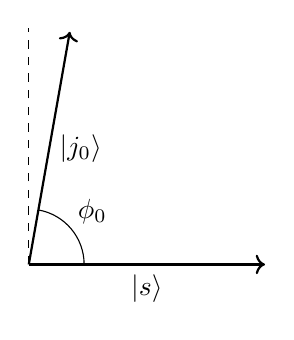
\begin{tikzpicture}
      \coordinate (O) at (0,0);
      \coordinate (P) at (3,0);
      \coordinate (Q) at (80:3);

      \draw[->, thick] (O) -- (P) node[midway,below] {$\ket{s}$};
      \draw[->, thick] (O) -- (Q) node[midway,right] {$\ket{j_0}$};
      \draw[dashed] (O) -- (0, 3);

      \draw pic["$\phi_0$",draw=black,angle radius=20,angle eccentricity=1.5]
    {angle = P--O--Q};
    \end{tikzpicture}
  \end{center}
  Then, by the inner product above, we have that $\phi_0 = \arccos(2^{-n/2})$.


  Note that $U_S$ and $U_f$ are \emph{reflections}, so $G$ is a rotation by some angle  $\alpha$.  In the plane containing $\ket{s}$ and $\ket{j_0}$, $U_f$ reflects on the line perpendicular to $\ket{j_0}$:

  \begin{center}
    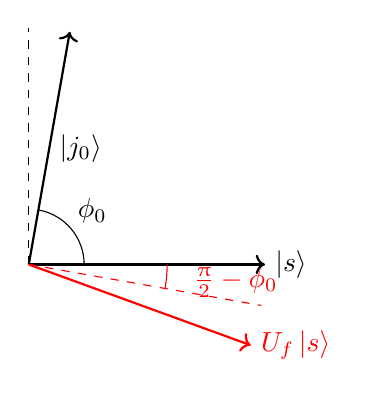
\begin{tikzpicture}
      \coordinate (O) at (0,0);
      \coordinate (P) at (3,0);
      \coordinate (Q) at (80:3);
      \coordinate (X) at (-10:3);
      \coordinate (Y) at (-20:3);

      \draw[->, thick] (O) -- (P) node[right] {$\ket{s}$};
      \draw[->, thick] (O) -- (Q) node[midway,right] {$\ket{j_0}$};
      \draw[dashed] (O) -- (0, 3);
      \draw[dashed, red] (O) -- (X);
      \draw[->, thick, red] (O) -- (Y) node[right] {$U_f \ket{s}$};

      \draw pic["$\phi_0$",draw=black,angle radius=20,angle eccentricity=1.5]
      {angle = P--O--Q};
      \draw pic["$\frac{\mpi}{2} - \phi_0$",draw,red,angle radius=50,angle eccentricity=1.5]
    {angle = X--O--P};
    \end{tikzpicture}
  \end{center}

  Similarly, $U_S$ reflects on the line perpendicular to $\ket{s}$.
  \begin{center}
    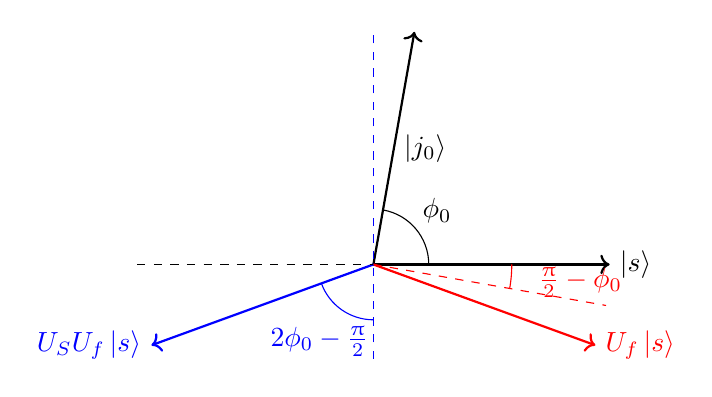
\begin{tikzpicture}
      \coordinate (O) at (0,0);
      \coordinate (P) at (3,0);
      \coordinate (R) at (0,-1.2);
      \coordinate (Q) at (80:3);
      \coordinate (X) at (-10:3);
      \coordinate (Y) at (-20:3);
      \coordinate (Z) at (200:3);

      \draw[->, thick] (O) -- (P) node[right] {$\ket{s}$};
      \draw[->, thick] (O) -- (Q) node[midway,right] {$\ket{j_0}$};
      \draw[dashed,blue] (R) -- (0, 3);
      \draw[dashed, red] (O) -- (X);
      \draw[->, thick, red] (O) -- (Y) node[right] {$U_f \ket{s}$};
      \draw[->, thick, blue] (O) -- (Z) node[left] {$U_SU_f \ket{s}$};
      \draw[dashed] (-3,0) -- (O);

      \draw pic["$\phi_0$",draw=black,angle radius=20,angle eccentricity=1.5]
      {angle = P--O--Q};
      \draw pic["$\frac{\mpi}{2} - \phi_0$",draw,red,angle radius=50,angle eccentricity=1.5]
      {angle = X--O--P};
      \draw pic["$2 \phi_0 - \frac{\mpi}{2}$",draw,blue,angle radius=20,angle eccentricity=1.7]
    {angle = Z--O--R};
    \end{tikzpicture}
  \end{center}

  Hence, we have:
  \begin{center}
    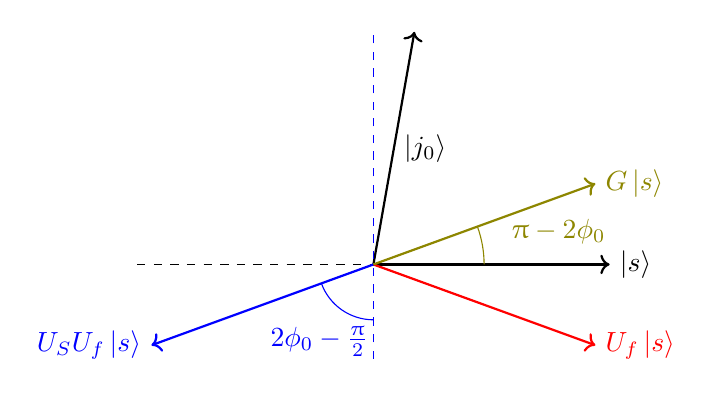
\begin{tikzpicture}
      \coordinate (O) at (0,0);
      \coordinate (P) at (3,0);
      \coordinate (R) at (0,-1.2);
      \coordinate (Q) at (80:3);
      \coordinate (X) at (-10:3);
      \coordinate (Y) at (-20:3);
      \coordinate (Z) at (200:3);
      \coordinate (W) at (200:-3);

      \draw[->, thick] (O) -- (P) node[right] {$\ket{s}$};
      \draw[->, thick] (O) -- (Q) node[midway,right] {$\ket{j_0}$};
      \draw[dashed,blue] (R) -- (0, 3);
      % \draw[dashed, red] (O) -- (X);
      \draw[dashed] (-3,0) -- (O);
      \draw[->, thick, red] (O) -- (Y) node[right] {$U_f \ket{s}$};
      \draw[->, thick, blue] (O) -- (Z) node[left] {$U_SU_f \ket{s}$};
      \draw[->, thick, olive] (O) -- (W) node[right] {$G \ket{s}$};

      % \draw pic["$\phi_0$",draw=black,angle radius=20,angle eccentricity=1.5]
      % {angle = P--O--Q};
      % \draw pic["$\frac{\mpi}{2} - \phi_0$",draw,red,angle radius=50,angle eccentricity=1.5]
      % {angle = X--O--P};
      \draw pic["$2 \phi_0 - \frac{\mpi}{2}$",draw,blue,angle radius=20,angle eccentricity=1.7]
      {angle = Z--O--R};
      \draw pic["$\mpi - 2 \phi_0$",draw,olive,angle radius=40,angle eccentricity=1.7]
      {angle = P--O--W};
    \end{tikzpicture}
  \end{center}

  Hence, $G$ is a rotation of $\alpha = \mpi - 2 \phi_0$.  Since $\phi_0$ is close to $\mpi/2$, we have that $\alpha$ is close to $0$.  So, we have:
  \begin{center}
    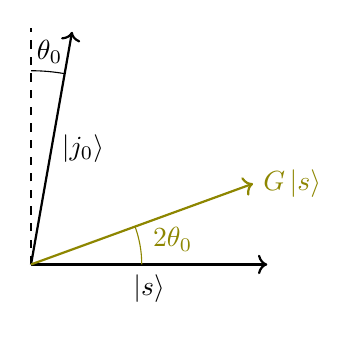
\begin{tikzpicture}
      \coordinate (O) at (0,0);
      \coordinate (P) at (3,0);
      \coordinate (R) at (0,-1.2);
      \coordinate (Q) at (80:3);
      \coordinate (X) at (-10:3);
      \coordinate (Y) at (-20:3);
      \coordinate (Z) at (200:3);
      \coordinate (W) at (200:-3);
      \coordinate (T) at (0,3);

      \draw[->, thick] (O) -- (P) node[midway,below] {$\ket{s}$};
      \draw[->, thick] (O) -- (Q) node[midway,right] {$\ket{j_0}$};
      \draw[dashed] (O) -- (0, 3);
      % \draw[dashed, red] (O) -- (X);
      % \draw[dashed] (-3,0) -- (O);
      % \draw[->, thick, red] (O) -- (Y) node[right] {$U_f \ket{s}$};
      % \draw[->, thick, blue] (O) -- (Z) node[left] {$U_SU_f \ket{s}$};
      \draw[->, thick, olive] (O) -- (W) node[right] {$G \ket{s}$};

      \draw pic["$\theta_0$",draw=black,angle radius=70,angle eccentricity=1.1]
      {angle = Q--O--T};
      % \draw pic["$\frac{\mpi}{2} - \phi_0$",draw,red,angle radius=50,angle eccentricity=1.5]
      % {angle = X--O--P};
      % \draw pic["$2 \phi_0 - \frac{\mpi}{2}$",draw,blue,angle radius=20,angle eccentricity=1.7]
      % {angle = Z--O--R};
      \draw pic["$2 \theta_0$",draw,olive,angle radius=40,angle eccentricity=1.3]
      {angle = P--O--W};
    \end{tikzpicture}
  \end{center}

  Therefore, the angle for $\ket{\psi_k} \idef G^k \ket{s}$ is $2k \theta_0$.  Hence, the angle between $\ket{\psi_k}$ and $\ket{j_0}$ is $\phi_0 - 2k \theta_0 = (2k+1) \phi_0 - k \mpi$.  Noting that
  \begin{itemize}

  \item $\phi_0 = \arccos(2^{-n/2})$,

  \item $\cos(x + \mpi/2) = -\sin(x)$, and

  \item $\mpi/2 - \arccos(\mpi/x) = \arcsin(x)$,

  \end{itemize}
  we have
  \begin{align*}
    \abs{\langle j_0 \mid \psi_k \rangle}^2
    &= \cos^2((2k+1)\phi_0 - k\mpi) \\
    &=\cos^2(-(2k+1)(\mpi/2 - \phi_0) + \mpi/2) \\
    &= \sin^2((2k+1) \arcsin(2^{-n/2})).
  \end{align*}


\end{proof}


\section{Quantum Fourier Transform}


(More of a quantum ``subroutine''.)


\begin{lemma}\label{lemma:expsum}
  Let $\zeta_N \idef \me^{2 \mpi \mi/N}$, with $N \geq 2$, and $a \in \R$.  Then we have
  \[
    \sum_{b=0}^{N-1} \zeta_N^{ab} =
    \begin{cases}
      N, & \text{if $a \in \Z$ and $a \equiv 0 \pmod{N}$}; \\
      0, & \text{if $a \in \Z$ and $a \not\equiv 0 \pmod{N}$}; \\
      \frac{{\left(\zeta_N^{a}\right)}^N - 1}{\zeta_N - 1}, & \text{if $a \not\in \Z$}.
    \end{cases}
  \]
\end{lemma}

\begin{proof}
  We have that $\zeta_N^a = 1$ if and only if $a \in \Z$ and $a \equiv 0 \pmod{N}$, in which case the result is trivial.  So, suppose that $\zeta_N^a \neq 1$.  Then:
  \[
    \sum_{b=0}^{N-1} {\left(\zeta_N^a\right)}^b = \frac{\zeta_N^{aN} - 1}{\zeta_N^a - 1}.
  \]
  If $a \in \Z$, then ${\left( \zeta_N^a \right)}^N = {\left( \zeta_N^N \right)}^a = 1$.
\end{proof}


\subsection{Discrete Fourier Transform}

\begin{definition}
  Let $f : \Z/{N}\Z \to \C$ and $\zeta \idef \me^{2\mpi\mi/N}$.  Then the \emph{Discrete Fourier Transform (DFT)}\index{Discrete Fourier Transform (DFT)} is defined as
  \[
    \ft(f)(z) \idef \frac{1}{\sqrt{N}} \sum_{x=0}^{N-1} \zeta_N^{xz} f(x).
  \]
\end{definition}

It decomposes $f$ into periodic functions.


\begin{proposition}
  We have:
  \begin{enumerate}

  \item $\ft$ is linear.

  \item \emph{Parseval identity}\index{Parseval identity}: if
    \[
      \langle f_1 \mid f_2 \rangle \idef \sum_{x=0}^{N-1} \bar{f}_1(x) f_2(x),
    \]
    then
    \[
      \langle \ft(f_1) \mid \ft(f_2) \rangle = \langle f_1 \mid f_2 \rangle,
    \]
    i.e., $\ft$ is unitary.

  \item Let $k \in \Z/{N}\Z$ and define the translation
    \[
      T_k(f)(x) \idef f(x - k).
    \]
    Then,
    \[
      T_k(\ft(f))(z) = \zeta_N^{kz} \ft(T_k(f))(z).
    \]

  \end{enumerate}
\end{proposition}

\begin{proof}
  Let $\zeta_k \idef \me^{2 \mpi \mi/k}$.   For Parseval's identity, using~\vref{lemma:expsum} we have:
  \begin{align*}
    \langle \ft(f_1) \mid \ft(f_2) \rangle
    &= \sum_{x=0}^{N-1} \left[ \frac{1}{\sqrt{N}} \sum_{x_1=0}^{N-1} \zeta_N^{-x_1x} \bar{f}_1(x_1)\right] \cdot \left[ \frac{1}{\sqrt{N}} \sum_{x_2=0}^{N-1} \zeta_N^{x_2x} \bar{f}_2(x_2)\right] \\
    &= \frac{1}{N} \sum_{x=0}^{N-1} \sum_{x_1, x_2=0}^{N-1} \zeta_N^{x(x_2 - x_1)} \bar{f}_1(x_1) f_2(x_2) \\
    &= \frac{1}{N} \sum_{x=0}^{N-1} \sum_{x_1=0}^{N-1} \bar{f}_1(x_1) f_2(x_1) \\
    &= \frac{1}{N} N \sum_{x_1=0}^{N-1} \bar{f}_1(x_1) f_2(x_1) \\
    &= \langle f_1 \mid f_2 \rangle.
  \end{align*}
\end{proof}


\subsection{Quantum Fourier Transform}

\begin{definition}
  Let $N \idef 2^n$, $\zeta_N \idef \me^{2 \mpi \mi/ N}$ and
  \[
    \ket{\psi} = \sum_{x=0}^{N-1} \psi(x) \ket{x}_n, \quad \psi : \Z/{N}\Z \to \C, \; \left\| \psi \right\| = 1.
  \]
  Then,
  \begin{align*}
    \qft \ket{\psi}
    &\idef \sum_{z=0}^{2^n-1}\ft(\psi)(z) \ket{z}_n \\
    &= \frac{1}{2^{n/2}}  \sum_{z=0}^{2^n - 1}\left[ \sum_{x=0}^{2^n-1} \zeta_{2^n}^{xz} \psi(x)\right] \ket{z}_n \\
    &= \frac{1}{2^{n/2}}  \sum_{x=0}^{2^n - 1} \psi(x) \left[ \sum_{z=0}^{2^n-1} \zeta_{2^n}^{xz} \ket{z}_n \right].
  \end{align*}
\end{definition}


In particular,
\[
  \qft \ket{x}_n = \frac{1}{2^{n/2}} \sum_{z=0}^{2^n-1} \zeta_{2^n}^{xz} \ket{z}_n
\]

Also note that
\[
  \qft^{-1} \ket{x}_n = \adj{\qft} \ket{x}_n = \frac{1}{2^{n/2}} \sum_{z=0}^{2^n-1} \zeta_{2^n}^{-xz} \ket{z}_n
\]

Indeed, using Lemma~\ref{lemma:expsum} again:
\begin{align*}
  \qft^{-1} \qft \ket{x}_n
  &=  \frac{1}{2^{n/2}} \sum_{z=0}^{2^n-1} \zeta_{2^n}^{xz} \left[  \frac{1}{2^{n/2}} \sum_{y=0}^{2^n-1} \zeta_{2^n}^{-yz} \ket{y}_n \right] \\
  &= \frac{1}{2^n} \sum_{y=0}^{2^n-1} \left[ \sum_{z=0}^{2^n - 1} \zeta_{2^n}^{z(x-y)}\right] \ket{y}_n \\
  &= \ket{x}_n.
\end{align*}

\begin{remark}
  One can compute $\ft(f)$ from $f$ using the \href{https://en.wikipedia.org/wiki/Fast_Fourier_transform}{fast Fourier transform} in $\mcal{O}(\log_2(N) N)$ time.
\end{remark}

\textbf{Fact:} There are quantum circuits for the quantum Fourier transform using $\mcal{O}(n^2) = \mcal{O}({(\log_2(N))}^2)$ gates, using only $1$-qubit gates and $\cnot$ gates.  (See Nielsen-Chuang pg.~217 for a ``good'' exact implementation.)


\begin{definition}
  \emph{Ancillas}\index{Ancillas} (or ancilla qubits) are extra qubits used in the quantum circuit.
\end{definition}


\subsection{Application: Adder Circuit}

We will need the following definition:

\begin{definition}\label{def:p-gate}
  We define the \emph{$P$ gate}\index{P gate@$P$ gate}:
  \[
    P(k) \ket{x}_n \idef \me^{2 \mpi \mi xk/2^{n}} \ket{x}_n.
  \]
\end{definition}


\begin{remark}
  \textbf{Careful!}  In qiskit we have
  \[
    P(\theta) = \begin{pmatrix*}[c]
      1 & 0 \\
      0 & \me^{\mi \theta}
    \end{pmatrix*}.
  \]
  So here, $P(k)$ corresponds to qiskit's $P(\mpi k)$!
\end{remark}


Hence, of $n=1$ we have that
\[
  P(k) = \begin{pmatrix*}[c]
    1 & 0 \\
    0 & \me^{\mpi \mi k}
  \end{pmatrix*} = \me^{-\mpi \mi k/2} \begin{pmatrix*}[c]
      \me^{-\mpi \mi k/2} & 0 \\
      0 & \me^{\mpi \mi k/2}
    \end{pmatrix*} = \me^{-\mpi \mi k/ 2} R_Z(\mpi k/2)
\]
Hence, we can easily implement the $P$ gates.  The circuit
\begin{center}
  \begin{quantikz}
    \lstick{$\ket{x_0}$} & \gate[5]{P(k)} & \\
    \lstick{$\ket{x_1}$} & & \\
    \lstick{$\ket{x_2}$} & &\\
    \setwiretype{n} \lstick{$\vdots \phantom{xi}$} & & \\
    \lstick{$\ket{x_{n-1}}$} & &
  \end{quantikz}
\end{center}
which, as a multi-qubit gate, is the same as
\begin{center}
  \begin{quantikz}
    \lstick{$\ket{x_0}$} & \gate{P(k/2^{n-1})} & \\
    \lstick{$\ket{x_1}$} & \gate{P(k/2^{n-2})} & \\
    \lstick{$\ket{x_2}$} & \gate{P(k/2^{n-3})}&\\
    \setwiretype{n} \lstick{$\vdots \phantom{xx}$} & \vdots & & \\
    \lstick{$\ket{x_{n-1}}$} & \gate{P(k)}&
  \end{quantikz}
\end{center}


\begin{definition}
  For $k \in \Z/{2^n}\Z$, define the \emph{plus $k$ adder}\index{plus $k$ adder}
  \[
    A_k \ket{x}_n \idef \ket{x + k}_n.
  \]
\end{definition}


\begin{align*}
  A_k \adj{\qft} \ket{x}_n
  &= \frac{1}{2^{n/2}} \sum_{z=0}^{2^n - 1} \zeta_{2^n}^{-xz} \ket{z + k}_n \\
  &= \frac{1}{2^{n/2}} \sum_{z=0}^{2^n - 1} \zeta_{2^n}^{-x(z-k)} \ket{z}_n \\
  &= \frac{1}{2^{n/2}} \zeta_{2^n}^{xk }\sum_{z=0}^{2^n - 1} \zeta_{2^n}^{-xz} \ket{z}_n \\
  &= \zeta_{2^n}^{xk} \adj{\qft} \ket{x}_n,
\end{align*}
i.e.,
\begin{equation}
  \label{eq:qftak}
  (\qft \circ A_k \circ \adj{\qft}) \ket{x}_n = \zeta_{2^n}^{xk} \ket{x}_n = P(k) \ket{x}_n,
\end{equation}
or
\begin{equation}\label{eq:ak}
  A_k = \adj{\qft} \circ P(k) \qft.
\end{equation}
(So, \emph{shift} is turned in to \emph{phase})


So, using~\cref{eq:ak}, and assuming that $\qft$ can be implemented, we can also implement $A_k$.

\begin{proof}
  Let
  \[
    x = x_0 + x_1 \cdot 2 + x_2 \cdot 2^2 + \cdots + x_{n-1} \cdot 2^{n-1} = \sum_{r=0}^{n-1} x_r 2^r.
  \]
  Then,
  \begin{equation}\label{eq:exp1}
    \exp\left(\frac{2 \mpi \mi}{2^n} xk \right) = \exp\left(k \mpi \mi \sum_{r=0}^{n-1} \frac{1}{2^{n-r-1}} x_r\right)
  \end{equation}

  Also, note that for a qubit $x_r$, we have
  \[
    R_Z(\theta) \ket{x_r} = \me^{-\mi \theta/2} \me^{\mi \theta x_r} \ket{x_r}.
  \]
  So,
  \[
    R_Z\left(\frac{k \mpi}{2^{n-1-r}}\right) \ket{x_r} = \exp\left(-\frac{k \mpi \mi}{2^{n-r}}\right) \cdot \exp\left(\frac{k \mpi \mi}{2^{n-1-r}} x_r\right) \ket{x_r}.
  \]

  Therefore:
  \begin{align*}
    \bigotimes_{r=0}^{n-1}R_Z\left(\frac{k \mpi} {2^{n-1-r}}\right) \ket{x_r}
    &= \bigotimes_{r=0}^{n-1} \exp\left(-\frac{k \mpi \mi}{2^{n-r}}\right) \cdot \exp\left(\frac{k \mpi \mi}{2^{n-1-r}} x_r\right) \ket{x_r} \\
    &= \left[\prod_{r=0}^{n-1} \exp\left(-\frac{k \mpi \mi}{2^{n-r}}\right) \cdot \prod_{r=0}^{n-1}  \exp\left(\frac{k \mpi \mi}{2^{n-1-r}} x_r\right)\right] \ket{x}_n \\
    &= \left[\exp\left(-\frac{k \mpi \mi}{2^n} \sum_{r=0}^{n-1} 2^r\right) \cdot \exp\left(k \mpi \mi \sum_{r=0}^{n-1}\frac{1}{2^{n-1-r}} x_r\right)\right] \ket{x}_n \\
    &= \exp\left(-\frac{(2^n-1) k \mpi \mi}{2^n}\right) \cdot \exp\left(\frac{2 \mpi \mi}{2^n} xk \right) \ket{x}_n \\
    &= \exp\left(-\frac{(2^n-1) k \mpi \mi}{2^n}\right) \cdot P(k) \ket{x}_n.
  \end{align*}
  So, indeed the last circuit gives, up to a global phase, the $P(k)$ gate.
\end{proof}


\section{Quantum Phase Estimation}

\subsection{Fejér States}

What happens if we replace $k \in \Z$ in $A(k)$ by some $k \in  \R$?

\begin{definition}
  For $n$ bits and $k \in \R$, define $\ket{k}_F\index[not]{ket k of F@$\ket{k}_F$}$, the \emph{$k$-th Fejér state}\index{Fejér state} as
  \begin{align*}
    \ket{k}_F
    &\idef \adj{\qft} \circ P(k) \circ \qft \ket{0}_n \\
    &= \sum_{z=0}^{2^n-1} \exp\left(\mpi \mi (1 - 1/2)(k - z)\right) \frac{\sin(\mpi(k-z))}{2^n \sin(\mpi (k-z)/ 2^n)} \ket{z}_n.
  \end{align*}
\end{definition}

Then, for $x \in \{0, 1, \ldots, 2^n-1\}$, we have
\[
  \prob(x \mid \ket{k}_F) = \abs{\langle x \mid k  \rangle_F}^2 = \frac{\sin^2(\mpi(k -x))}{4^n \sin^2(\mpi(k-x)/2^n)},
\]
the \emph{Fejér kernel}\index{Fejér kernel}.

\Vref{fig:fejer_kernel} shows the graph of the Fejér kernel
\[
   \frac{\sin^2(\mpi(k -x))}{4^n \sin^2(\mpi(k-x)/2^n)}
\]
for $n = 5$ and $k = 17.3$.

\begin{figure}
  \centering
  \includegraphics[scale=0.6]{fejer_kernel.jpg}
  \caption{Ferjér kernel for $k=17.3$ and $n=5$.}
  \label{fig:fejer_kernel}
\end{figure}


If we let $k = x_0 + r$, where $x_0 = \lfloor k \rceil$, so $r \in [-1/2, 1/2]$, then
\[
  \prob(x_0 \mid \ket{k}_F) = \frac{\sin^2(\mpi r)}{4^n \sin^2(\mpi r/2^n)} \geq \frac{4}{\mpi^2} \approx 0.41,
\]
and in fact
\[
   \prob(\lfloor x \rfloor \mid \ket{k}_F) +  \prob(\lceil x \rceil \mid \ket{k}_F) \geq \frac{8}{\mpi^2} \approx 0.82.
\]


\subsection{Quantum Phase Estimator/Digitizer}

Let $\mcal{H}$ be the Hilbert space of $m$-qubit states.  Given
\begin{itemize}

\item an implementation of an unitary operator $U$;

\item an \emph{eigenstate} $\ket{\psi} \in \mcal{H}$ of $U$, with $U \ket{\psi} = \me^{2 \pi \mi \theta} \ket{\psi}$, with $0 \leq \theta < 1$;

\end{itemize}
we want to find or estimate $\theta$.

\begin{remark}
  Note that $\ket{\psi} \sim \me^{2 \pi \mi \theta} \ket{\psi}$, so physically there is no difference (and hence asking for $\theta$, as is, is not a proper question). On the other hand, when we have a controlled gate $CU$ given by
  \[
    CU( \ket{a} \ket{\psi}) = \ket{a} U^a \ket{\psi} \quad \text{(for $a \in \F_2$)},
  \]
  i.e.,
  \[
    CU( \alpha \ket{0} \ket{\psi} + \beta \ket{1} \ket{\psi}) = \alpha \ket{0} \ket{\psi} + \beta \me^{2 \pi \mi \theta} \ket{1} \ket{\psi},
  \]
  then $\theta$ is relevant.
\end{remark}

\begin{definition}
  We define the $n$-qubit \emph{quantum phase estimator}\index{quantum phase estimator} $\qpe \ket{x}_n\ket{\psi}$ as:
  \begin{center}
    \begin{quantikz}
      \lstick{$\ket{x_0}$} &  & \gate[5, nwires=4]{H} & \ctrl{5}  &  &  &  &  & \cdots &  & \gate[5, nwires=4]{\qft} & \meter{} &  \\
      \lstick{$\ket{x_1}$} &   &  &  &  & \ctrl{4} &  &  & \cdots &  &  & \meter{} &  \\
      \lstick{$\ket{x_2}$} & &  &  &  &  & \ctrl{3} &  & \cdots &  &  & \meter{} &  \\
      \setwiretype{n} \lstick{$\ \vdots \ $} & & &  &  &  &  &  & \cdots & &  & \vdots  &  \\
      \lstick{$\ket{x_{n-1}}$} &  &  &  &  &  &  &  & \cdots & \ctrl{1} &  & \meter{} &  \\
      \lstick{$\ket{\psi}$} &  &  & \gate{U} &  & \gate{U^2} & \gate{U^{2^2}} &  & \cdots & \gate{U^{2^{n-1}}} &  &  &
    \end{quantikz}
  \end{center}
\end{definition}

We then have that
\[
  \qpe \ket{x}_n \ket{\psi} = \ket{x + 2^n \theta}_F \ket{\psi}.
\]
In particular,
\[
  \qpe \ket{0}_n \ket{\psi} = \ket{2^n \theta}_F \ket{\psi}.
\]
Hence, measuring the first $n$ qubits, we get either $\lfloor 2^n \theta \rfloor$ or $\lceil 2^n \theta \rceil$ with probability at least $82\%$.  Pick the most likely $x_{\theta} \in \Z$ and then $\theta \approx x_{\theta} / 2^n$.


\section{Shor's Algorithm}\label{sec:shor}

Given $a \in \Z/{N}\Z$, with $\gcd(a, N) = 1$, f the order of $a \in {\Z/{N}\Z}^{\times}$.  Classical methods are \href{https://en.wikipedia.org/wiki/Time_complexity#Superpolynomial_time}{superpolynomial} in $\log_2(N)$, with $\mcal{O}\left({(1 + \epsilon)}^{\log_2(N)}\right)$ for any $\epsilon > 0$.


Let $n \idef \lceil \log_2(N) \rceil$.  Shor showed that one can implement
\[
  U_a \ket{x}_{n} =
  \begin{cases}
    \ket{ax \mmod{N}}_n, & \text{if $0 \leq x < N$}; \\
    \ket{x}_n, & \text{if $N \leq x < 2^n$};
  \end{cases}
\]
with $\mcal{O}(n^2)$ gates and ancillas.  Then, one can use $\qpe$ to compute the order.


\subsection{The Spectrum of $U_a$}

Suppose $\gcd(a, N) = 1$.  Then for $x \geq N$, we have that $\ket{x}_n$ is an eigenstate of $U_a$, with eigenvalue $1$.

Now, let $r \idef \abs{a}$.  Then, clearly we have that $x^r - 1$ is the minimal polynomial of $U_a$, so the eigenvalues of $U_a$ are of the form $\me^{2 \mpi \mi k /r}$, for $k \in \{0, 1, \ldots , r-1\}$.

Let $\zeta_s \idef \me^{2 \mpi \mi/r}$ and
\[
  \ket{\phi_k} \idef \frac{1}{\sqrt{r}} \sum_{s=0}^{r-1} \zeta_r^{ks} \ket{a^s \mmod N}
\]
for $k \in \{0, 1, \ldots, r-1\}$.  Then,
\begin{align*}
  U_a \ket{\phi_k} &= \zeta_r^k \ket{\phi_k}; \\
  \langle \phi_{k_1} \mid \phi_{k_2} \rangle &= \delta_{k_1, k_2}; \\
  \frac{1}{\sqrt{r}} \sum_{k=0}^{r-1} \ket{\phi_k} &= \ket{1}_n = \ket{100 \ldots 0}.
\end{align*}


Consider the circuit:
\begin{center}
  \begin{quantikz}%[wire types={q,q,n,q,q,q,n,q}]
    \lstick[4]{$\ket{0}_{2n}$} &  & \gate[8]{\qpe_{U_a}} & \meter{} &\\
    &  &  & \meter{} & \\
    \setwiretype{n} & \ \vdots\ & & \vdots & \\
    &   &  &  \meter{} & \\
    \lstick[4]{$\ket{1}_{n}$} & & & \rstick[4]{$\ket{a^k \mmod 2^n}$ (for some $k$)}\\
    & & & \\
    \setwiretype{n} & \vdots & & \\
    & & &
  \end{quantikz}
\end{center}
Since $U_{a^{2^k}}$ needs $\mcal{O}(n^2)$ gates, we have that $\qpe_{U_a}$ needs $\mcal{O}(n^3)$ gates.

Now:
\begin{align*}
  \ket{a ; n} &\idef \qpe_{U_a} (\ket{0}_{2n} \ket{1}_n) \\
  &= \qpe_{U_a}\left( \ket{0}_{2n}   \frac{1}{\sqrt{r}} \sum_{k=0}^{r-1} \ket{\phi_k} \right) \\
  &=\frac{1}{\sqrt{r}} \sum_{k=0}^{r-1} \qpe_{U_a}\left( \ket{0}_{2n}\ket{\phi_k} \right) \\
  &=\frac{1}{\sqrt{r}} \sum_{k=0}^{r-1} \ket{2^{2n}k/r}_{F}\ket{\phi_k}
\end{align*}

So, for $0 \leq y < 2^{2n}$, we have
\begin{equation}\label{eq:ketan}
  \prob(y \mid \ket{a; n}) = \frac{1}{r} \sum_{k=0}^{r-1}  \abs{\langle y \mid 2^{2n}k/r \rangle_F}^2.
\end{equation}
Now, for each $k$, the most likely $y$, i.e., the value that makes $\abs{\langle y \mid 2^{2n}k/r \rangle_F}^2$ the largest, is the integer $y$ closest to $2^{2n}k/r$, in which case we must have
\[
  \abs{y - 2^{2n} \frac{k}{r}} \leq \frac{1}{2} \quad \Longleftrightarrow \quad \abs{\frac{y}{2^{2n}} - \frac{k}{r}} \leq \frac{1}{2^{2n+1}}.
\]


\begin{lemma}\label{lemma:approx}
  Let $n \idef \lceil \log_2(N) \rceil \geq 2$.  Then, for a fraction $k/r$ with $0 \leq k < r < N$, there is a unique $y \in \{0, 1, 2, \ldots, 2^{2n}-1\}$ such that
  \[
    \abs{\frac{y}{2^{2n}} - \frac{k}{r}} < \frac{1}{2^{2n+1}}.
  \]

  Conversely, given $y \in \{0, 1, 2, \ldots, 2^{2n}-1\}$, if there exists $k/r$ with $0 \leq k < r < N$ such that
  \[
    \abs{\frac{y}{2^{2n}} - \frac{k}{r}} < \frac{1}{2^{2n+1}},
  \]
  then this fraction $k/r$ is unique.
\end{lemma}

\begin{proof}
  We have
  \[
    0 = \frac{0}{2^{2n}} \leq \frac{k}{r} \leq \frac{N-1}{N} = 1 - \frac{1}{N} \leq 1 -  \frac{1}{2^n} < 1 - \frac{2}{2^{2n}} = \frac{2^{2n} - 2}{2^{2n}},
  \]
  i.e.,
  \[
     \frac{0}{2^{2n}} \leq \frac{k}{r} < \frac{2^{2n} - 2}{2^{2n}},
  \]
  So, there $y_0 \in \{0, 1, \ldots, 2^{2n}-2\}$ such that
  \[
    \frac{y_0}{2^{2n}} \leq \frac{k}{r} < \frac{y_0+1}{2^{2n}}.
  \]
  Thus, taking $y$ as either $y_0$ or $y_0 + 1$, and hence $y \in \{0, 1, 2, \ldots, 2^{2n} -1 \}$, we can obtain
  \[
    \abs{\frac{y}{2^{2n}} - \frac{k}{r}} \leq \frac{1}{2} \frac{1}{2^{2n}} = \frac{1}{2^{2n+1}}.
  \]
  On the other hand, the only way we get the equality is if
  \[
    \frac{k}{r} = \frac{2y_0 + 1}{2^{2n+1}},
  \]
  which would imply that $2^{2n+1} \mid r$ (since the fraction on the right is reduced), which is a contradiction, as $r \leq N \leq 2^{n}$.  Thus, we have that there exists $y$ with
  \[
    \abs{\frac{y}{2^{2n}} - \frac{k}{r}} < \frac{1}{2^{2n+1}}.
  \]

  Now, suppose that we also have $y' \neq y$, with $y' \in \{0, 1, 2, \ldots, 2^{2n}-1\}$, such that
  \[
    \abs{\frac{y'}{2^{2n}} - \frac{k}{r}} <  \frac{1}{2^{2n+1}}.
  \]
  Then,
  \[
     \frac{1}{2^{2n}} \leq \abs{\frac{y'}{2^{2n}} - \frac{y}{2^{2n}}} \leq \abs{\frac{y'}{2^{2n}} - \frac{k}{r}} + \abs{\frac{y}{2^{2n}} - \frac{k}{r}} < \frac{1}{2^{2n}},
   \]
   which is a contradiction.

   \bigskip

   For the second part, assume that $k/r \neq k'/r'$, within the corresponding ranges and such that
   \[
     \abs{\frac{y}{2^{2n}} - \frac{k}{r}} < \frac{1}{2^{2n+1}}, \quad     \abs{\frac{y}{2^{2n}} - \frac{k'}{r'}} < \frac{1}{2^{2n+1}}.
   \]
   Then, by the triangle inequality, we have that
   \[
     \frac{1}{N^2} < \frac{1}{rr'} \leq \frac{\abs{kr'-k'r}}{rr'} = \abs{\frac{k}{r} - \frac{k'}{r'}} < \frac{1}{2^{2n}},
   \]
   i.e., $N > 2^n$, or $\log_2(N) > n = \ceil{\log_2(N)}$, a contradiction.
\end{proof}

So, by \cref{eq:ketan}, the first part of \cref{lemma:approx} and the previous section, when measuring the resulting $\ket{a; n}$, the first $2n$ qubits will correspond to some $y$ close to some $k/r$.  (If $y/2^{2n}$ is not close to any $k/r$, the probability in \cref{eq:ketan} is quite small!)  Then, by the second part, this $k/r$ is unique with
\[
  \abs{\frac{y}{2^{2n}} - \frac{k}{r}} < \frac{1}{2^{2n + 1}}.
\]

We then can use \emph{continued fractions} to find $r$: remember that there are $a_1, a_2, a_3, \ldots \in \Z$ such that
\[
  \frac{y}{2^{2n}} = [a_1, a_2, a_3, \ldots] \idef  \cfrac{1}{a_1 + \cfrac{1}{a_2 + \cfrac{1}{a_3 + \cdots}}}.
\]
Then, if $[a_1, a_2, \ldots, a_n] = p_n/q_n$, then
\[
  \abs{\frac{y}{2^{2n}} - \frac{p_n}{q_n}} < \frac{1}{2q_n^2}
\]
Therefore, we use continued fractions until we get $\frac{1}{2q_n^2} \leq \frac{1}{2^{2n+1}}$ (with $q_n < N$ still).  Then, we must have
\[
  \frac{k}{r} = \frac{p_n}{q_n},
\]
We can then try to compute $a^{q_n}$.  If we get $1$, we found the order $r$!  If not, we can try some small multiples that are still less than $N$.  If that also fails, we can repeat the method of $\abs{a^{q_n}}$.  Alternatively, we could do another reading, which would likely give us another $y$ with close $y/2^{2n}$ to (likely) another $k/r$, and find a new fraction $p_t'/q_t'$ using continued fractions.  If $q_t's$ also does not work, but it is different from $q_n$, we know that $\mathrm{lcm}(q_n, q_t') \mid r$.


\section{Quantum Data Access Oracles}

In classical data we often need functions $f : \F_2^n \to \F_2^d$, e.g., for lists, dictionaries, etc.  How do we implement these on a quantum computer?

One possibility is to construct a \emph{data access oracle}\index{data access oracle}:
\[
  U_f \ket{x}_n \ket{0}_d \idef \ket{x}_n \ket{f(x)}_d.
\]
(Note we do not specify $U_f \ket{x}_n \ket{y}_d$ for $y \neq 0$.)  (How do we construct $U_f$?)

Alternatively, we could use \emph{diagonal unitaries}\index{diagonal unitaries}:
\[
  \mathcal{D}_f \ket{x}_n \idef \me^{2 \pi \mi/2^d f(x)} \ket{x}_n
\]
(seeing $f(x)$ as the integer corresponding to the one given by its binary representation).  (How do we construct $\mathcal{D}_f$?)


\section{Implementing $U_f$}

\subsection{Select QROM}

QROM means that $f$ is in the circuit, not in the quantum computer.

\begin{definition}
  Given $x_0 \in \F_2^n$, we define the gate $C_{x_0}^n X\index[not]{c x zero X@$C_{x_0}^n X$}$ by:
  \[
    C_{x_0}^n X \ket{x}_n \ket{y}_1 =
    \begin{cases}
      \ket{x}_n \ket{y}_1,& \text{if $x \neq x_0$,} \\
      \ket{x}_n \ket{y + 1}_1, & \text{if $x=x_0$.}
    \end{cases}
  \]
  If $x_0 = x_{0,0} + x_{0,1} \cdot 2 + c_{0,2} \cdot 2^2 + \cdots + c_{0,n-1} \cdot 2^{n-1}$, then we have the $C_{x_0}^n X$ is given by
  \begin{center}
    \begin{quantikz}
      \lstick[4]{$\ket{x}_n$} & \gate{X^{1-x_{0,0}}} & \ctrl{2} &  \gate{X^{1-x_{0,0}}} & \\
      & \gate{X^{1-x_{0,1}}} & \ctrl{1} &  \gate{X^{1-x_{0,1}}} & \\
      \setwiretype{n} & \vdots & \vdots & \vdots \\
      & \gate{X^{1-x_{0,n-1}}} & \ctrl{1} &  \gate{X^{1-x_{0,n-1}}} & \\
      \lstick{$\ket{y}_1$} & & \targ{} & &
    \end{quantikz}
  \end{center}
\end{definition}

The circuit above works by simply making $\ket{x_0}_n \mapsto \ket{11\cdots 1}$ in the first step (and $\ket{x}$ does not give $\ket{111\cdots 1}$ when $x \neq x_0$), then the control gates flips $\ket{0}$ to $\ket{1}$, and then undoing the first step.

\begin{remark}
  Note that $C_{x_0}^n X$ is the same $U_f$ for
  \[
    f(x) =
    \begin{cases}
      0,& \text{if $x \neq x_0$,} \\
      1,& \text{if $x = x_0$}.
    \end{cases}
  \]
\end{remark}

Then, to implement $C_f$, we just use various $C_{x_0}^n X$ flipping the corresponding qubits in the output.  (See example below.)



\begin{example}
  Consider
  \begin{align*}
    f(0, 0) &= (1, 0), & f(1,0) &= (1, 1), \\
    f(0, 1) &= (0, 0), & f(1,1) &= (0, 1).
  \end{align*}
  Here is $C_f$:
  \begin{center}
    \begin{quantikz}[]
    \lstick{$x_0$} & \gate{X} & \ctrl{1} & \gate{X} \slice{$f(0,0)$}&        & \ctrl{3} &          & & & \ctrl{3} \slice{$f(1,1)$} &\\
      \lstick{$x_1$} & \gate{X} & \ctrl{1} & \gate{X}          & \gate{X} & \ctrl{1}  & \gate{X} & \slice{$f(1,0)$} & \slice[label style={pos=1, anchor=north}]{$f(0,1)$} & \ctrl{1}  & \\
     \lstick{$y_0$} &          & \targ{}  &                   &          & \targ{}  &          & &&          &\\
     \lstick{$y_1$} &           &         &                   &          & \targ{}  &          & && \targ{}  &
    \end{quantikz}
  \end{center}
\end{example}

\begin{remarks}
  \begin{enumerate}

  \item This naive implementation often have many cancellations of consecutive $X$ gates.

  \item The state of the art implementation can be done with $\mathcal{O}(d2^n)$ $H$, $S$, and $CX$ gates, and $\mathcal{O}(2^n)$ $T$ gates.

  \item This select QROM is efficient when $f$ has either few non-zero entries or if its \emph{unstructured}.

  \item The size of the ancilla in this case is just $d$, so it is \emph{shallow} (few ancillas).

  \item On the other hand, it is \emph{long}.

  \item Much better if the data is sparse, with many zeros.

  \end{enumerate}
\end{remarks}


\subsection{Swap QRAM}

QRAM means that the quantum computer knows $f$, not the circuit.

\begin{definition}
  The \emph{swap gate}\index{swap gate} $\swpg\index[not]{swap@$\swpg$}$ is defined as
  \[
    \swpg \ket{x}_1 \ket{y}_1 \idef \ket{y}_1 \ket{x}_1.
  \]
  It is represented by:
  \begin{center}
    \begin{quantikz}
      \lstick{$\ket{x}$} & \swap{1} & \rstick{$\ket{y}$} \\
      \lstick{$\ket{y}$} & \swap{-1} & \rstick{$\ket{x}$}
    \end{quantikz}
  \end{center}

  The \emph{controlled swap gate}\index{controlled swap gate} $\cswp$ is defined as
  \[
    \cswp \ket{xyz} =
    \begin{cases}
      \ket{xyz}, & \text{if $x = 0$}, \\
      \ket{xzy}, & \text{if $x = 1$}. \\
    \end{cases}
  \]
  It is represented as
  \begin{center}
    \begin{quantikz}
      & \ctrl{2}  & \\
      & \swap{1}  &  \\
      & \swap{-1} &
    \end{quantikz}
  \end{center}
\end{definition}

Note that $\swpg$ can be implemented as
\begin{center}
  \begin{quantikz}
    & \targ{} & \ctrl{1} & \targ{} &\\
    & \ctrl{-1} & \targ{} & \ctrl{-1} &
  \end{quantikz}
\end{center}
and $\cswp$ as
\begin{center}
  \begin{quantikz}
    & & \ctrl{1} & & \\
    & \targ{} & \ctrl{1} & \targ{} &\\
    & \ctrl{-1} & \targ{} & \ctrl{-1} &
  \end{quantikz}
\end{center}


\begin{example}
  Let's give an example of a QRAM swap with $n=2$ and $d=1$:
  \begin{align*}
    f(0, 0) &= 0 , & f(1,0) &= 1 \\
    f(0, 1) &= 1 , & f(1,1) &= 1
  \end{align*}
  We first create the possible outputs in the last $2^n$ qubits, corresponding to $f(0,0)$, $f(1,0)$, $f(0,1)$, and $f(1,1)$ respectively:
  \begin{center}
    \begin{quantikz}
      \lstick{$\ket{x_0}$} & &\\
      \lstick{$\ket{x_1}$} & &\\
      \lstick{output}   & & \\
      \lstick{$f(0,0)$} & & \\
      \lstick{$f(1,0)$} & \gate{X} & \\
      \lstick{$f(0,1)$} & \gate{X} & \\
      \lstick{$f(1,1)$} & \gate{X} &
    \end{quantikz}
  \end{center}

  If the last qubit of the input is $1$, we swap the correct output to the places where the last qubits were $0$:
  \begin{center}
    \begin{quantikz}
      \lstick{$\ket{x_0}$} & & & &\\
      \lstick{$\ket{x_1}$} & & \ctrl{3} & \ctrl{4} &\\
      \lstick{output}   & & & & \\
      \lstick{$f(0,0)$} & & \swap{2} & &\\
      \lstick{$f(1,0)$} & \gate{X}\slice{} & & \swap{2} &\\
      \lstick{$f(0,1)$} & \gate{X} & \swap{-2} & &\\
      \lstick{$f(1,1)$} & \gate{X} & & \swap{-2}&
    \end{quantikz}
  \end{center}
  This makes the correct output $f(x_0, x_1)$ to be in the spots of $f(x_0,0)$.

  Then, if the first qubit is $1$, we swap the correct output to where the first qubits were $0$:
  \begin{center}
    \begin{quantikz}
      \lstick{$\ket{x_0}$} & & & & \ctrl{4} & \\
      \lstick{$\ket{x_1}$} & & \ctrl{3} & \ctrl{4}\slice{} & &\\
      \lstick{output}   & & & & &\\
      \lstick{$f(0,0)$} & & \swap{2} & & \swap{1} &\\
      \lstick{$f(1,0)$} & \gate{X}\slice{} & & \swap{2} &  \swap{-11}&\\
      \lstick{$f(0,1)$} & \gate{X} & \swap{-2} & & &\\
      \lstick{$f(1,1)$} & \gate{X} & & \swap{-2}& &
    \end{quantikz}
  \end{center}
  This makes then the correct output $f(x_0, x_1)$ to be in the spot of $f(0,0)$.  At this point we could just measure the fourth qubit (corresponding to $f(0,0)$), but we could do a final swap to put it in the third spot:
  \begin{center}
    \begin{quantikz}
      \lstick{$\ket{x_0}$} & & & & \ctrl{4} \slice{} & &\\
      \lstick{$\ket{x_1}$} & & \ctrl{3} & \ctrl{4}\slice{} & & &\\
      \lstick{output}   & & & & & \swap{1} &  \rstick{$\ket{f(x_0, x_1)}$}\\
      \lstick{$f(0,0)$} & & \swap{2} & & \swap{1} & \swap{-1} & \\
      \lstick{$f(1,0)$} & \gate{X}\slice{} & & \swap{2} &  \swap{-11}& & \\
      \lstick{$f(0,1)$} & \gate{X} & \swap{-2} & & && \\
      \lstick{$f(1,1)$} & \gate{X} & & \swap{-2}& &
    \end{quantikz}
  \end{center}
\end{example}

\begin{example}
  Here is a more complex example (without the final swap), the same as above:
  \begin{align*}
    f(0, 0) &= (1, 0), & f(1,0) &= (1, 1), \\
    f(0, 1) &= (0, 0), & f(1,1) &= (0, 1).
  \end{align*}

  The steps are the same:
  \begin{enumerate}

  \item set the correct outputs for $f(x_0, y_0)$ in their respective spots;

  \item place the result of $f(x_0, y_0)$ in the spots for $f(x_0, 0)$;

  \item place the result of $f(x_0, y_0)$ in the spots for $f(0, 0)$.

  \end{enumerate}

  We have:
  \begin{center}
    \begin{quantikz}
      \lstick{$\ket{x_0}$} & & & & & & \ctrl{4} & \ctrl{5} &\\
      \lstick{$\ket{x_1}$} & & \ctrl{5} & \ctrl{6} & \ctrl{7} & \ctrl{8} & & &\\
      \lstick[2]{$f(0,0)$} & \gate{X}\slice{} & \swap{4} & & & & \swap{2} & & \rstick[2]{$\ket{f(x_0,x_1)}_2$}\\
      & & & \swap{4} & & & & \swap{2} &\\
      \lstick[2]{$f(1,0)$} & \gate{X} & & & \swap{2} & &\swap{-2} & &\\
      &  \gate{X} & & & & \swap{4} & & \swap{-2} &\\
      \lstick[2]{$f(0,1)$} & & \swap{-4} & & & & & &\\
      & & & \swap{-4} & & & & &\\
      \lstick[2]{$f(1,1)$} & & & & \swap{-4} & & & &\\
      &  \gate{X} & & & & \swap{-4}\slice{} & & &
    \end{quantikz}
  \end{center}
\end{example}



\begin{remark}
  The ancilla needed in this method needs $2^n d$ qubits, so it is very \emph{wide}, but is shallow (not long).  Even the state of the art has $\mathcal{O}(d 2^n)$ gates.  (Much better if the data is sparse, with many zeros.)
\end{remark}

\subsection{Select-Swap}

One can combine the two methods.  We can select $k$ qubits at the end of the input of $f$ to obtain a function $g : \F_2^{n-k} \to \F_2^{d2^k}$:
\[
  g(x_0, \ldots , x_{n-k-1}) \idef (g_1(x_0, \ldots , x_{n-k-1}), \ldots, g_{2^k-1}(x_0, \ldots , x_{n-k-1})),
\]
where $g_i : \F_2^{n-k} \to \F_2^d$ is defined as
\[
  g_i(x_0, \ldots , x_{n-k-1}) \idef f(x_0, \ldots ,x_{n-k-1}, \text{``$k$ binary representation of $i$''}).
\]

We can then use the select method for each $g_i$ and then swap to get the correct answer in the $f(0,0, \ldots , 0)$ spot.

This makes it so we need $d2^{k}$ ancillas, compared to the $d2^n$ of the swap method.


\begin{example}
  Consider
  \begin{align*}
    f(0,0,0,0) &= (0,1,0) & f(1, 0, 0, 0) &= (1, 0, 0), & f(0,1,0,0) &= (0,0,0) & f(1, 1, 0, 0) &= (1,1,0), \\
    f(0,0,1,0) &= (0,0,1) & f(1, 0, 1, 0) &= (0, 0, 1), & f(0,1,1,0) &= (0,1,0) & f(1, 1, 1, 0) &= (0,1,0), \\
    f(0,0,0,1) &= (0,0,0) & f(1, 0, 0, 1) &= (1, 1, 0), & f(0,1,0,1) &= (1,1,1) & f(1, 1, 0, 1) &= (0,0,0), \\
    f(0,0,1,1) &= (1,1,1) & f(1, 0, 1, 1) &= (0, 1, 0), & f(0,1,1,1) &= (0,0,0) & f(1, 1, 1, 1) &= (0,1,0).
  \end{align*}
  For $k=2$, we have:
  \begin{align*}
    g_0(0, 0) &= (0,1,0), & g_0(1,0) &= (1, 0, 0), \\
    g_0(0, 1) &= (0,0,0), & g_0(1,1) &= (1, 1, 0),
  \end{align*}
  and
  \begin{align*}
    g_1(0, 0) &= (0,0,1), & g_1(1,0) &= (0, 0, 1), \\
    g_1(0, 1) &= (0,1,0), & g_1(1,1) &= (0, 1, 0),
  \end{align*}
  and
  \begin{align*}
    g_2(0, 0) &= (0,0,0), & g_2(1,0) &= (1, 1, 0), \\
    g_2(0, 1) &= (1,1,1), & g_2(1,1) &= (0, 0, 0),
  \end{align*}
  and
  \begin{align*}
    g_3(0, 0) &= (1,1,1), & g_3(1,0) &= (0, 1, 0), \\
    g_3(0, 1) &= (0,0,0), & g_3(1,1) &= (0, 1, 0).
  \end{align*}

  We then get:
  \begin{center}
    \tiny
    \begin{quantikz}[row sep=3ex]
      \lstick{$\ket{x_0}$} & \gate{X} & \ctrl{15} & \gate{X}\slice{} & & \ctrl{1} && & \gate{X} & \ctrl{1} &\gate{X}\slice{} & \ctrl{1} \slice{} & \\
      \lstick{$\ket{x_1}$} & \gate{X} & \ctrl{14} & \gate{X} & \gate{X} & \ctrl{13} &\gate{X}\slice{} & && \ctrl{11} && \ctrl{13} &\\
      \lstick{$\ket{x_2}$} & && && && &&&&&\\
      \lstick{$\ket{x_3}$} & && && && &&&&&\\
      \lstick[3]{$g_0$}&& & && \targ{} & & &&&& \targ{} & \\
       && \targ{}& &&&& &&&& \targ{} &\\
       && & &&&& &&&& &\\
      \lstick[3]{$g_1$} && & &&&& &&&& &\\
       && & &&&& && \targ{} && \targ{} &\\
       && \targ{}& && \targ{} && &&&& &\\
      \lstick[3]{$g_2$} && & && \targ{} && && \targ{} &&&\\
       && & && \targ{} && && \targ{} &&&\\
       && & &&&& && \targ{} &&&\\
       \lstick[3]{$g_3$}&& \targ{}& &&&& &&&&&\\
       && \targ{} && & \targ{} && &&&&\targ{} &\\
       && \targ{} & &&&& &&&&&
    \end{quantikz}
  \end{center}
  followed by the swaps:
  \begin{center}
    \tiny
    \begin{quantikz}
      \lstick{$\ket{x_0}$}\slice{} & & & & & & & & &&\\
      \lstick{$\ket{x_1}$} & & & & & & & & &&\\
      \lstick{$\ket{x_2}$} & & & & && & \ctrl{2} & \ctrl{3} & \ctrl{4} &\\
      \lstick{$\ket{x_3}$} & \ctrl{1} & \ctrl{2} & \ctrl{3} & \ctrl{4} & \ctrl{5} & \ctrl{6}\slice{} & & &&\\
      \lstick[3]{$g_0$} & \swap{6} & & & & & & \swap{3} &&&\rstick[3]{$f(x_0,x_1,x_2,x_3)$}\\
      && \swap{6} & & & && & \swap{3} &&\\
      && & \swap{6} & & & & & & \swap{3} &\\
      \lstick[3]{$g_1$} & & & & \swap{6} & & & \swap{-3} &&&\\
      &&&&& \swap{6} & && \swap{-3} &&\\
      &&&&& & \swap{6}&&& \swap{-3} &\\
      \lstick[3]{$g_2$} & \swap{-6} &&&&&&&&&\\
      && \swap{-6} &&&&&&&& \\
      && & \swap{-6} &&&&&&&\\
      \lstick[3]{$g_3$} & &&&\swap{-6} &&&&&&\\
      && &&& \swap{-6}&&&&&\\
      && &&&&\swap{-6}&&&&
    \end{quantikz}
  \end{center}
\end{example}


So,
\[
  U_f^{\mathrm{Sel-Swap}} \ket{x}_n \ket{0}_{d2^k} = \ket{x}_n \ket{f(x)}_d \ket{\text{garbage}}_{d(2^k - 1).}
\]

The total cost is the cost of the $2^k$ select, plus the swap of $k$.  So, the total gate cost is $\mathcal{O}(d2^k)$ and width $\mathcal{O}(2^{n-k} + d2^k)$.  Choosing $k \approx n/2$, we get $\mathcal{O}\left(\sqrt{d2^n}\right)$.

\begin{remark}
  If we restrict to $H$, $T$, $S$, and $CX$, then the $T$ cost is only $\mathcal{O}\left( \sqrt{d2^n} \right)$.  (A bit higher on the others.)
\end{remark}

\subsection{Diagonal Unitary}

Given some $\theta : \F_2^n \to [0, 1)$, we might want
\[
  U_\theta \ket{x}_n = \me^{2 \mpi \mi \theta(x)} \ket{x}_n.
\]
We can approximate it using data access oracles.

If $\epsilon > 0$ is the error, and in binary
\[
  \theta(x) = 0.\underbrace{y_0 y_1 \cdots y_d}_{\idef \theta_d(x)} y_{d+1} y_{d+2} \cdots
\]
then $\theta_d : \F_2^n \to \F_2^d$ and $\abs{\me^{2 \mpi \mi \theta(x)} - \me^{2 \mpi \mi \theta_d(x)}} \leq c/2^d < \epsilon$, for some constant $c$.  So, we need $d \approx \log_2(1/\epsilon) + \mathcal{O}(1)$.

So, with the data access oracle $U_{\theta_d}$, we can make
\begin{center}
  \begin{quantikz}
    \lstick{$\ket{x}_n$} & \gate[2]{U_{\theta_d}} & & \gate[2]{U_{\theta_d}^{-1}} & \meter{} & \\
    \lstick{$\ket{0}_d$} & & \gate{P(1)} & & &
  \end{quantikz}
\end{center}
where the $P$ gate is given as in Definition~\ref{def:p-gate}:
\[
  P(1) \ket{x}_n \idef P(1/2^{n-1}) \ket{x_0} \otimes P(1/2^{n-2}) \ket{x_1} \otimes \cdots \otimes P(1) \ket{x_{n-1}}.
\]


This works since we get
\begin{align*}
  \ket{x}_n \ket{0}_d
  &\mapsto \ket{x}_n \ket{\theta_d(x)}_d \\
  &\mapsto \ket{x}_n \me^{2\pi \mi \theta_d(x)/2^{d}} \ket{\theta_d(x)}_d \\
  &= \me^{2\pi \mi \theta_d(x)/2^{d}} \ket{0}_n \ket{\theta_d(x)}_d \\
  &\mapsto \left(\me^{2\pi \mi \theta_d(x)/2^{d}} \ket{0}_n\right) \ket{0}_d \\
  &\approx \left(\me^{2\pi \mi \theta(x)} \ket{0}_n\right) \ket{0}_d.
\end{align*}


One more observation.  Let:

\begin{definition}
  Given $\theta : \F_2^n \to [0, 1)$ as above, a \emph{multiplexer}\index{multiplexer} of type $Y$ (or $X$, or $Z$):
  \[
    R_Y(\theta) \ket{x}_n \ket{\psi}_1 = \ket{x}_n R_Y(\theta(x)) \ket{\psi}_1,
  \]
  with
  \[
    R_Y(\theta) = \begin{pmatrix*}[c]
      \cos(\theta/2) & -\sin(\theta/2) \\
      \sin(\theta/2) & \cos(\theta/2)
    \end{pmatrix*}
  \]
  as in Section~\ref{sec:rotations}.
\end{definition}

These can also be done with data access oracles!



\section{Quantum State Preparation}


Given $\{ \psi_x \st x \in \F_2^n \} \subseteq \C^{2n}$, can we construct $U_\psi$ such that $U_\psi \ket{0}_n = \ket{\psi}_n$?

Here is a construction that is not always the best, but always works and often is the best.  We construct it inductively.

\begin{enumerate}

\item Let $\psi_x = \me^{2 \pi\mi \theta(x)} \rho_x$, where $\rho_x \idef \abs{\psi_x}$.  Then, $\ket{\psi} = U_{\theta} \ket{\rho}$.  (We can choose, for instance, $\theta(x) = 0$ if $\rho_x = 0$.)  Since we can get $U_\theta$, we may assume without loss of generality that $\psi_x \geq 0$ for all $x$.

\item Let
  \begin{align*}
    \ket{\psi}_n
    &= \sum_{x \in \F_2^n} \psi_x \ket{x}_n \\
    &= \sum_{y \in \F_2^{n-1}} \psi_{y,0} \ket{y}_{n-1} \ket{0} +  \psi_{y,1} \ket{y}_{n-1} \ket{1} \\
    &= \ket{\chi}_{n-1} \otimes \left( C(y) \ket{0} +  S(y) \ket{1} \right),
  \end{align*}
  where
  \begin{align*}
    \ket{\chi}_{n-1} &\idef \sum_{y \in \F_2^{n-1}} \sqrt{\psi_{y,0}^2 + \psi_{y,1}^2} \ket{y}_{n-1}, \\
    C(y) &\idef \frac{\psi_{y,0}}{\sqrt{\psi_{y,0}^2 + \psi_{y,1}^2}}, \\
    S(y) & \idef \frac{\psi_{y,1}}{\sqrt{\psi_{y,0}^2 + \psi_{y,1}^2}}.
  \end{align*}
  (Note that if $\psi_{y,0} = \psi_{y,1} = 0$ above, we can just skip the term in the summation.)

  Note that since $C(y), S(y) \geq 0$ and ${C(y)}^2 + {S(y)}^2 = 1$, there exists a unique $\theta(y) \in [0, \mpi]$ such that $C(y) = \cos(\theta(y)/2)$ and $S(y) = \sin(\theta(y)/2)$.

  Also,
  \[
    \langle \chi \mid \chi \rangle = \sum_{y \in \F_2^{n-1}} \psi_{y,0}^2 + \psi_{y,1}^2 = \sum_{x \in \F_2^n} \psi_x^2 = \langle \psi \mid \psi \rangle = 1.
  \]


\item If we can prepare $\ket{\chi}_{n-1}$, we can prepare $\ket{\psi}_n$, as
  \[
    \ket{\psi}_n = (\idt \otimes R_Y(\theta)) \ket{\chi}_{n-1} \ket{0}_1.
  \]

  \item Finally, we can prepare any initial $1$-qubit state, exactly as above, as given $\ket{\psi}_1 = a \ket{0} + b \ket{1}$ there is some $\theta$ such that $R_Y(\theta) \ket{0} = \ket{\psi}_1$.

\end{enumerate}


\begin{example}
  Let's look at the $n=2$ case, with $\psi_x \geq 0$:
  \begin{align*}
    \ket{\psi}
    &= \psi_{0,0} \ket{00} + \psi_{1,0} \ket{10} + \psi_{0,1} \ket{01} + \psi_{1,1} \ket{11} \\
    &= \ket{0} \left( \psi_{0,0} \ket{0} + \psi_{0,1} \ket{1} \right) + \ket{1} \left( \psi_{1,0} \ket{0} + \psi_{1,1} \ket{1} \right) \\
    &= \sqrt{\psi_{0,0}^2 + \psi_{0,1}^2} \ket{0} \left( \frac{\psi_{0,0}}{\sqrt{\psi_{0,0}^2 + \psi_{0,1}^2}} \ket{0} + \frac{\psi_{0,1}}{\sqrt{\psi_{0,0}^2 + \psi_{0,1}^2}} \ket{1} \right) \\
    &\phantom{=} + \sqrt{\psi_{1,0}^2 + \psi_{1,1}^2} \ket{1} \left( \frac{\psi_{1,0}}{\sqrt{\psi_{1,0}^2 + \psi_{1,1}^2}} \ket{0} + \frac{\psi_{1,1}}{\sqrt{\psi_{1,0}^2 + \psi_{1,1}^2}} \ket{1}\right).
  \end{align*}
  Then,
  \begin{align*}
    \cos\left( \frac{\theta(0)}{2} \right) &\idef  \frac{\psi_{0,0}}{\sqrt{\psi_{0,0}^2 + \psi_{0,1}^2}}, \\
    \cos\left( \frac{\theta(1)}{2} \right) &\idef  \frac{\psi_{1,0}}{\sqrt{\psi_{1,0}^2 + \psi_{1,1}^2}}, \\
    \cos\left( \frac{\phi}{2} \right) &\idef  \sqrt{\psi_{0,0}^2 + \psi_{0,1}^2}.
  \end{align*}

  Hence, we have:
  \begin{multline*}
    \ket{\psi} = \cos\left( \frac{\phi}{2} \right) \ket{0} \left( \cos\left( \frac{\theta(0)}{2} \right) + \sin\left( \frac{\theta(0)}{2} \right)\right) \\
    + \sin\left( \frac{\phi}{2} \right) \ket{0} \left( \cos\left( \frac{\theta(1)}{2} \right) + \sin\left( \frac{\theta(1)}{2} \right)\right).
  \end{multline*}

  So, we need:
  \begin{center}
    \begin{quantikz}
      \lstick{$\ket{0}$} & \gate{R_Y(\phi)} & \gate{X} & \ctrl{1} & \gate{X} & \ctrl{1} &\\
      \lstick{$\ket{1}$} & & & \gate{R_Y(\theta(0))} & & \gate{R_Y(\theta(1))} &
    \end{quantikz}
  \end{center}
\end{example}


\section{Quantum (Hamiltonian) Simulations}

Quantum systems modeled by Hilbert spaces $\mathcal{H}$.

\textbf{Important operator:} $H$, the Hamiltonian.  $H$ is a self-adjoint operator, so it has real spectrum, and it can be diagonalized with an eigenbasis that is orthonormal.

Physical meanings:
\begin{enumerate}

\item The spectrum of $H$ are the possible energies of the system.  For every energy value $E$, there is a quantum state $\ket{\psi_E}$ such that $H \ket{\psi_E} = E \ket{\psi_E}$.

\item The \emph{time dependent Schr\"odinger equation}\index{time dependent Schr\"odinger equation}: the \emph{initial value problem}
  \begin{align*}
    \ket{\psi(t_0)} &= \ket{\psi_0}, \\
    \frac{\md}{\md t} \ket{\psi(t)} &= - i \hbar H \ket{\psi(t)},
  \end{align*}
  where $\hbar$ is an universal constant.  ($H$ is assumed here to not depend on time.)  The solution is
  \[
    \ket{\psi(t)} = \exp \left( - \frac{\mi}{\hbar} t H \right) \ket{\psi_0}.
  \]

\end{enumerate}


We want to simulate the time evolution!


\begin{itemize}

\item[\emph{Input:}] $\ket{\psi_0}$, $H$, and $t$.

\item[\emph{Output:}] $\ket{\psi(t)}$, or at least an approximation.

\end{itemize}

We have the formula, but it is hard to compute.


\begin{definition}
  For an operator $U$, a \emph{singular value}\index{singular value} of $U$ is the square root of an eigenvalue of the self-adjoint operator $\adj{U} U$. (The eigenvalues are then necessarily real and non-negative).  Then, the \emph{operator norm}\index{operator norm} of $U$, denoted by $\left\| U \right\|$, is the maximal singular value of $U$.
\end{definition}

\begin{remark}
  If $U$ is diagonalizable, with real eigenvalues (like self-adjoint matrices), then $\left\| U \right\|$ is the maximal absolute value of the eigenvalues of $U$.
\end{remark}

\begin{definition}
  A Hamiltonian on $n$ qubits can be \emph{efficiently simulated}\index{efficiently simulated} if there exists a quantum circuit $U_{t, \epsilon}$, for any small $t, \epsilon > 0$, such that
  \[
    \left\| \exp(-\mi t H/\hbar) - U_{t, \epsilon}\right\| = \max \left(\spec \left(\exp(-\mi t H/\hbar)\right)\right) < \epsilon,
  \]
  and $U$ is made out of $\Poly(n, t, 1/\epsilon)$ gate.
\end{definition}


\begin{example}
  Consider:
  \[
    H = \sum_{r=1}^{m} H_r,
  \]
  where each $H_r$ is acting on at most $k \ll n$ qubits.  (These are called \emph{$k$-local Hamiltonians}\index{k-local Hamiltonians@$k$-local Hamiltonians}.)
\end{example}


\section{Trotter's Formula}

\begin{theorem}[Trotter]
  We have
  \[
  \exp\left( - \frac{\mi}{\hbar} (H_1 + H_2 + \cdots + H_m )t\right) = \lim_{\ell \to \infty} {\left( \exp\left( - \frac{\mi H_1}{\hbar \frac{t}{\ell}} \right) \exp\left( - \frac{\mi H_2}{\hbar \frac{t}{\ell}} \right) \cdots \exp\left( - \frac{\mi H_m}{\hbar \frac{t}{\ell}} \right)\right)}^\ell
\]
\end{theorem}


So, fix $\ell > 0$: if you can construct $\exp(-\mi H_r / \hbar \cdot t/\ell)$ for each $r$, then we have:
\[
  \exp\left( - \frac{\mi}{\hbar} Ht \right) \approx  {\left( \exp\left( - \frac{\mi H_1}{\hbar \frac{t}{\ell}} \right) \exp\left( - \frac{\mi H_2}{\hbar \frac{t}{\ell}} \right) \cdots \exp\left( - \frac{\mi H_m}{\hbar \frac{t}{\ell}} \right)\right)}^\ell.
\]

(See more details at the \href{https://people.maths.bris.ac.uk/~csxam/teaching/qc2020/lecturenotes.pdf}{Montanaro's Notes}.)


\begin{example}
  Suppose that $H_r = \alpha_r \left( \sigma_{r,0} \otimes \sigma_{r,1} \otimes \cdots \otimes \sigma_{r, n-1} \right)$, with $\alpha_r \in \R$ and $\sigma_{r,s} \in \{\idt, X, Y, Z\}$.  $H = \sum_{r=1}^m H_r$ is $k$-local if and only if the number of non-identities is less than or equal to $k$ in each $H_r$.

  \emph{Claim:} $\exp\left( -\mi H_r t / \hbar \right)$ can be constructed (exactly, not approximated) using a single $R_Z$ rotation, $\mathcal{O}(1)$ $1$-qubit gates, and $\mathcal{O}(n)$ $CX$ gates.

  The idea of the proof is that
  \[
    Y = SH Z H\adj{S}, \qquad X = HZH,
  \]
  (so $X$, $Y$, and $Z$ are conjugates of each other).  So,
  \begin{align*}
    \exp\left( - \frac{\mi H_r}{\hbar} t \right)
    &= \exp\left( - \frac{\mi}{\hbar}\alpha_r(\sigma_{r,0} \otimes \sigma_{r,1} \otimes \cdots \otimes \sigma{r, n-1})t \right) \\
    &= \exp\left({- \frac{\mi \alpha_r t}{\hbar} R \sigma \adj{R}}\right) \\
    &= R \exp\left( - \frac{\mi \alpha_r t}{\hbar} \sigma \right) \adj{R},
  \end{align*}
  where $R$ is an unitary operator made of factors of $H$, $S$, and $\sigma$ is a tensor products of $\idt$'s and $Z$'.

  Then, we have
  \[
    \exp\left( -\mi t Z^{\otimes c} \right) =
  \]
\end{example}



\section{Quantum Error Correction}


\begin{definition}
  A \emph{$[n,k,d]$-code}\index{nkd code@$[n,k,d]$-code} is an error correcting code with $n$ physical bits, i.e., the number of bits in the code words (or the dimension of the space of code words), $k$ is the number of logical bits, i.e., the number of bits of a decoded code word, and minimum distance $k$, i.e., the number of bit flips needed to get from a code word to another.
\end{definition}


\begin{remarks}
  \begin{enumerate}

  \item We must have $k < n$.

  \item Also, $d \leq n$ and we can correct $\lfloor (d-1)/2 \rfloor$ errors.

  \end{enumerate}
\end{remarks}

Errors in quantum computing are more complicated, even if all errors are one-qubit errors, as besides bit-flips, we also might have phase-flips.

Moreover, they can occur at any stage, e.g., quantum state preparation, applying Pauli gates, measuring, or even while idling!  Note that we need to recover the \emph{superposition}, not just the $0$/$1$ state.

A $1$-qubit error $U_{\epsilon}$, with $\left\| U_{\epsilon} -\idt \right\| < \mathcal{O}(\epsilon)$.  For example,
\[
  U_{\epsilon} = \sqrt{1 - \epsilon^2} \idt + \epsilon \left( aX + bY + cZ \right),
\]
for some $a$, $b$, and $c$ fixed.  (So, $X$ gives a bit-flip, $Z$ gives a phase-flip, and $Y$ gives both.)

So, we might start with $\ket{0}$ and end with $U_{\epsilon} \ket{0}$.

\subsection{Quantum $3$-Qubit Code}

We have one logical qubit with three physical one:
\begin{align*}
  \ket{0_L} &\idef \ket{000}, \\
  \ket{1_L} &\idef \ket{111}.
\end{align*}
The code states have the form:
\[
  \ket{\psi_L} = \alpha \ket{000} + \beta \ket{111}, \qquad |\alpha|^2 + |\beta|^2 = 1.
\]
We need something such that:
\begin{center}
  \begin{quantikz}
    \lstick[3]{$\ket{\psi_L}$} & \gate[3]{\text{error}} & \gate[3]{\text{?}} & \rstick[3]{$\ket{\psi_l}$ (with high prob.)} \\
    &&& \\
    &&&
  \end{quantikz}
\end{center}

Here is the idea:
\begin{center}
  \begin{quantikz}
    \lstick[3]{$\ket{\psi_L}$} & \gate[3]{U_{\epsilon}}\slice{} & \ctrl{3} & & & & &\\
    &&& \ctrl{2} && \ctrl{3} &&\\
    &&&& &&\ctrl{2} & \\
    \ket{0} &&\targ{} & \targ{} & &&& \meter{} & \rstick{$s_0$}\\
    \ket{0} &&&&  &\targ{} & \targ{} & \meter{} & \rstick{$s_1$}
  \end{quantikz}
\end{center}

(These $s_0$ and $s_1$ are \href{https://en.wikipedia.org/wiki/Decoding_methods#Syndrome_decoding}{syndromes}.)

Here $U_{\epsilon}$ is the error.  (We write it as gate, but it is unintentional, unlike the gates we apply to a circuit.)  Suppose we get $\ket{abc}$ after the error (so, after the barrier/slice in the figure), then $s_0 = a + b$ and $s_1 = b + c$. \emph{Assuming} that no errors occurred in the ancilla, we have
\begin{align*}
  s_0 = 1 \quad &\Longleftrightarrow \quad a \neq b, \\
  s_1 = 1 \quad &\Longleftrightarrow \quad b \neq c.
\end{align*}
Since we want $a = b = c$, if either $s_0$ or $s_1$ is $1$, we have an error.  More precisely,
\begin{center}
  \begin{tabular}{c|cccc}
    \toprule
    $(s_0, s_1)$ & $(0, 0)$ & $(1, 0)$ & $(0, 1)$ & $(1, 1)$ \\
    \textbf{Equalities} & $a=b=c$ & $a \neq b = c$ & $a = b \neq c$ & $b \neq a = c$ \\
    \textbf{Error} & None & $a$ is off & $c$ is off & $b$ is off \\
    \textbf{Fix} & None & $X$ on $\ket{x_0}$ & $X$ on $\ket{x_2}$ & $X$ on $\ket{x_1}$\\
    \bottomrule
  \end{tabular}
\end{center}


To make it concrete, let's assume that the error is that one of the of the qubits are chosen, e.g., the first one, and $R_X(\epsilon)$ is acted on it, remembering that $R_X(\epsilon) = \me^{-\mi \epsilon X/2} = \cos\left(\epsilon/2 \right) \idt - \mi \sin(\epsilon/2) X$.  So, $U_{\epsilon} = R_X(\epsilon) \otimes \idt \otimes \idt$:

\begin{center}
  \begin{quantikz}
    \lstick[3]{$\ket{\psi_L}$} & \gate{R_X(\epsilon)}\slice{} & \ctrl{3} & & & & &\\
    &&& \ctrl{2} && \ctrl{3} &&\\
    &&&& &&\ctrl{2} & \\
    \ket{0} &&\targ{} & \targ{} & &&& \meter{} & \rstick{$s_0$}\\
    \ket{0} &&&&  &\targ{} & \targ{} & \meter{} & \rstick{$s_1$}
  \end{quantikz}
\end{center}


Now,
\begin{align*}
  (R_X(\epsilon) \otimes \idt \otimes \idt) \ket{\psi}
  &= (R_X(\epsilon) \otimes \idt \otimes \idt)(\alpha \ket{000} + \beta \ket{111})  \\
  &= \alpha(R_X(\epsilon) \ket{0}) \ket{00} + \beta (R_X(\epsilon) \ket{1}) \ket{11} \\
  &= \alpha \cos(\epsilon/2) \ket{000} - \alpha \mi \sin(\epsilon/2) \ket{100} \\
  &\qquad + \beta \cos(\epsilon/2) \ket{111} - \beta \mi \sin(\epsilon/2) \ket{011}.
\end{align*}

So, in the whole process, we get:
\begin{align*}
  \ket{\psi}_3 \ket{00}
  &\mapsto \alpha \cos(\epsilon/2) \ket{000}\ket{00} - \alpha \mi \sin(\epsilon/2) \ket{100}\ket{00} \\
  &\qquad + \beta \cos(\epsilon/2) \ket{111}\ket{00} - \beta \mi \sin(\epsilon/2) \ket{011}\ket{00} \\
  &\mapsto \alpha \cos(\epsilon/2) \ket{000}\ket{00} - \alpha \mi \sin(\epsilon/2) \ket{100}\ket{10} \\
  &\qquad + \beta \cos(\epsilon/2) \ket{111}\ket{00} - \beta \mi \sin(\epsilon/2) \ket{011}\ket{10} \\
  & = \cos(\epsilon/2)\left(\alpha \ket{000} + \beta \ket{111} \right) \ket{00} \\
  &\qquad - \mi \sin(\epsilon/2) \left( \alpha \ket{100}+ \beta \ket{011} \right)\ket{10}.
\end{align*}

We then measure the last two qubits.  For small $\epsilon$, it is likely we measure $s_0 = 0$ (with probability $\cos^2(\epsilon/2)$).  And, in the case of our example, we are sure that $s_1$ will measure zero.

If we get $s_0 = 0$, then we get the correct $\alpha \ket{000} + \beta \ket{111}$ back.  If we get $s_0 = 1$, we get $\alpha \ket{100} + \beta \ket{011}$ back, and we need to apply an $X$-gate to the first qubit.

\begin{remark}
  Note that if there are two qubit-flips, the process above will ``correct'' incorrectly.  More importantly, it does not correct $Z$-errors.
\end{remark}


\subsection{Correcting $Z$-Errors}

Note that $Z=HXH$, and so
\[
  Z \ket{+} = \ket{-}, \qquad Z \ket{-} = \ket{+}.
\]

Thus, one can use a similar idea as above, where we apply $H = H^{-1}$ to make it into an $X$-error, and then another $H$ to restore.  More precisely, let
\begin{align*}
  \ket{\tilde{0}_L} &\idef \ket{+++} = H^{\otimes 3} \ket{000}, \\
  \ket{\tilde{1}_L} &\idef \ket{---} = H^{\otimes 3} \ket{111},
\end{align*}
and given $\ket{\tilde{\psi}_L}$, we can detect $Z$-errors with:

\begin{center}
  \begin{quantikz}
    \lstick[3]{$\ket{\tilde{\psi}_L}$} & \gate[3]{U_{\epsilon}}\slice{} & \gate{H} & \ctrl{3} & \gate{H} &&& & & && &&\\
    &&&&& \gate{H} & \ctrl{2} && \ctrl{3} & \gate{H} &&&&\\
    &&&&&&& &&& \gate{H} & \ctrl{2} & \gate{H} &\\
    \ket{0} && &\targ{}& && \targ{} & &&&&&& \meter{} & \rstick{$s_0$}\\
    \ket{0} &&&&&&&  &\targ{} &&& \targ{} && \meter{} & \rstick{$s_1$}
  \end{quantikz}
\end{center}

The basic circuit is:
\begin{center}
  \begin{quantikz}
   \lstick{$x$} & \gate{H} & \ctrl{1} & \gate{H} & \\
   \lstick{$c$} & & \targ{} & &
  \end{quantikz}
\end{center}

Then, the idea is that $Z \ket{\pm} = Z \ket{\mp}$, so

\begin{center}
  \begin{tikzcd}[cramped, sep=8ex]
    \ket{+} \ket{0} \arrow[r, mapsto, "H \otimes \idt"] &\ket{0} \ket{0} \arrow[r, mapsto, "\cnot"] &\ket{0} \ket{0} \arrow[r, mapsto, "H \otimes \idt"] &\ket{+} \ket{0} \\
    \ket{-} \ket{0} \arrow[r, mapsto, "H \otimes \idt"] &\ket{1} \ket{0} \arrow[r, mapsto, "\cnot"] &\ket{1} \ket{1} \arrow[r, mapsto, "H \otimes \idt"] &\ket{-} \ket{0}
  \end{tikzcd}
\end{center}

On the other hand, note that the circuit above is equivalent to
\begin{center}
  \begin{quantikz}
    \lstick{$x$} & & \targ{} & & \\
    \lstick{$c$} & \gate{H} & \ctrl{-1} & \gate{H} &
  \end{quantikz}
\end{center}

Indeed, for $x \in \{0,1\}$, we have:
\begin{align*}
  \ket{+} \ket{x}
  & \mapsto \ket{+} \ket{{(-1)}^x} \\
  &= \frac{1}{2} \left[ \left( \ket{0} + \ket{1} \right) \otimes  \left( \ket{0} + {(-1)}^x \ket{1} \right) \right] \\
  &= \frac{1}{2} \left[ \ket{00} + \ket{10} + {(-1)}^x \ket{01} + {(-1)}^x \ket{11} \right] \\
  &\mapsto \frac{1}{2} \left[ \ket{00} + \ket{10} + {(-1)}^x \ket{11} + {(-1)}^x \ket{01} \right] \\
  &= \ket{+} \ket{{(-1)}^x} \\
  &\mapsto \ket{+} \ket{x},
\end{align*}
and
\begin{align*}
  \ket{-} \ket{x}
  & \mapsto \ket{-} \ket{{(-1)}^x} \\
  &= \frac{1}{2} \left[ \left( \ket{0} - \ket{1} \right) \otimes  \left( \ket{0} + {(-1)}^x \ket{1} \right) \right] \\
  &= \frac{1}{2} \left[ \ket{00} - \ket{10} + {(-1)}^x \ket{01} - {(-1)}^x \ket{11} \right] \\
  &\mapsto \frac{1}{2} \left[ \ket{00} - \ket{10} + {(-1)}^x \ket{11} - {(-1)}^x \ket{01} \right] \\
  &= \ket{-} \ket{{(-1)}^{x \oplus 1}} \\
  &\mapsto \ket{-} \ket{x \oplus 1}.
\end{align*}

This second representation can save some gates, since $H^2 = \idt$, in the implementation of the error detection.  For instance, the full circuit above becomes:

\begin{center}
  \begin{quantikz}
    \lstick[3]{$\ket{\tilde{\psi}_L}$} & \gate[3]{U_{\epsilon}}\slice{} & & \targ{} & & &&& &\\
    &&& \targ{} && & \targ{} & &&\\
    &&&&& & \targ{} && &\\
    \ket{0} && \gate{H} & \ctrl{-3} & \gate{H} & && & \meter{} & \rstick{$s_0$} \\
    \ket{0} &&&&& \gate{H} & \ctrl{-3} & \gate{H} & \meter{} & \rstick{$s_1$}
  \end{quantikz}
\end{center}



\subsection{Shor's $9$-Qubit Code}

(See also:\href{https://abdullahkhalid.com/qecft/qec-intro/shor-code/}{A Methods Focused Guide to Quantum Error Correction and Fault-Tolerant Quantum Computation} by Abdullah Khalid.)

Shor's $9$-qubit code is a combination of a $3$-qubit repetition code to correct $X$ errors and $Z$ errors.  We have:
\begin{align*}
  \ket{\shr{0}_L} &\idef {\left[ \frac{1}{\sqrt{2}} \left( \ket{000} + \ket{111} \right) \right]}^{\otimes 3}, \\
  \ket{\shr{1}_L} &\idef {\left[ \frac{1}{\sqrt{2}} \left( \ket{000} - \ket{111} \right) \right]}^{\otimes 3}.
\end{align*}

Each bundle of three can be used to correct $Z$-errors, and the subbundles of three can be used to correct $X$-errors.  It can correct arbitrary $1$-qubit errors.  It can also correct one $X$ and one $Z$ error on any different groups of $3$ (bundles).

So, Shor's code is a $[[9, 1, 3]]$ code.

An alternative point of view: the physical Hilbert space is $\mathcal{H}_{\mathrm{phys}} = {(\C^2)}^{\otimes 9}$ while the logical Hilbert space is $\mathcal{H}_{\mathrm{logical}} = \sspan\left( \ket{\shr{0}_L}, \ket{\shr{1}_L} \right)$.  We also can describe $\mathcal{H}_{\mathrm{logical}}$ as the simultaneous $+1$-eigenspace of the group
\[
  S \idef \left\langle Z_{0,1}, Z_{1,2}, Z_{3, 4}, Z_{4, 5}, Z_{6, 7}, Z_{7,8}, X_{0,1,2,3,4,5}, X_{3,4,5,6,7,8} \right\rangle
\]
where $Z_{i,j}$ is the tensor product of nine $\idt$ and $Z$, with $Z$ appearing in the $i$-th and $j$-th components only (counting from $0$), and similarly for the $X_{i, j, \ldots}$ above.  In other words,
\[
  \mathcal{H}_{\mathrm{logical}} = \stab(S) \idef \{ \ket{\psi} \in \mathcal{H}_{\mathrm{phys}} \st A \ket{\psi} = \ket{\psi} \text{ for all } A \in S\}.
\]

Note that $S$ is commutative and for all $A \in S$, we have that $A^2 = \idt$.  In fact, one can prove that $S \cong \F_2^8$.

\begin{definition}
  A group $S = \langle P_1, P_2, \ldots , P_k \rangle$ is an $n$-qubit \emph{stabilizer group}\index{stabilizer group} if
  \begin{enumerate}

  \item $P_i$ is a tensor product of $\idt$'s, $X$'s, and $Z$'s, i.e., it is a \emph{Pauli string}\index{Pauli string};

  \item $S$ is commutative (i.e., $P_i P_j = P_j P_i$ for all $i$ and $j$).  (This is needed for the sake of diagonalization.)

  \end{enumerate}

  Note that for all $P \in S$, then, we have that $P^2 = \idt$.

  We then define
  \[
    \mathcal{H}_{\mathrm{logical}}^S \idef \stab(S) \idef \{ \ket{\psi} \in \mathcal{H}_{\mathrm{phys}} \st P \ket{\psi} = \ket{\psi} \text{ for all } P \in S\}.
  \]
\end{definition}

\begin{remark}
  If $S = \langle P_1, P_2, \ldots, P_k \rangle$, with the $P_i$'s \emph{independent}\index{independent} (i.e., removing any $P_i$ would yield a different group, or, alternatively, if $S$ as an $\F_2$-vector space has dimension $k$, with the $P_i$'s forming a basis), then $\mathcal{H}_{\mathrm{logical}}^S$ is a Hilbert space of dimension $2^{n-k}$.
\end{remark}


Remembering that $P_i$ is a tensor product of $\idt$, $X$, and $X$, then if, say, an $X$-error $U$ occurs on a qubit for which $P_i$ has a $Z$ factor, then $P_i U = -U P_i$, since $XZ = -ZX$.  Then, for $\ket{\psi_L} \in \mathcal{H}_{\mathrm{logical}}^S$, we have
\[
  P_i (U \ket{\psi_L}) = -U (P_i \ket{\psi_L}) = - (U \ket{\psi_L}).
\]
So, the erroneous state is not a $+1$ eigenvector of $P_i$, but a $-1$ eigenvector!

Thus, if we can measure eigenvalues of $P_i$, we can get syndromes for errors.

Then, back to Shor's Code, with $Z_{i,j}$ we can detect $X$ errors on $i$ or $j$.

\begin{center}
  \begin{quantikz}
    \lstick{$i$} & \ctrl{2} & & \\
    \lstick{$j$} & & \ctrl{1} & \\
    \lstick{s} & \targ{} & \targ{} &
  \end{quantikz}
\end{center}


Similarly, with $X_{i,j,k,l,m,n}$ we can detect $Z$ errors on the corresponding indices.

\begin{center}
  \begin{quantikz}
    \lstick{$i$} & & \targ{} & & \\
    \lstick{$j$} & & \targ{} & & \\
    \lstick{$k$} & & \targ{} & & \\
    \lstick{$l$} & & \targ{} & & \\
    \lstick{$m$} & & \targ{} & & \\
    \lstick{$m$} & & \targ{} & & \\
    \lstick{$s$} & \gate{H} & \ctrl{-6} & \gate{H} & \\
  \end{quantikz}
\end{center}


\begin{remark}
  Shor's $9$-qubit code is ``low quality'', since we need $9$ qubits for a single logical qubit and still can fix only one error, but it illustrates important ideas.

  There are quantum \emph{low density parity check} (LDPC) that are $[[n,k,d]]$ with $k \approx n(1 - \epsilon_1)$ and $d \approx n(1 - \epsilon_2)$, which scale well.
\end{remark}


\subsection{$5$ Qubit Code}

Here is an example of a more efficient code, using only $5$ qubits per logical qubit:

\begin{example}
  Consider $S \idef \langle P_1, P_2, P_3, P_4 \rangle$ with:
  \begin{align*}
    P_1 &\idef \idt \otimes X \otimes Z \otimes Z \otimes X ,\\
    P_2 &\idef X \otimes \idt \otimes X \otimes Z \otimes Z ,\\
    P_3 &\idef Z \otimes X \otimes \idt \otimes X \otimes Z, \\
    P_4 &\idef X \otimes Z \otimes Z \otimes X \otimes \idt.
  \end{align*}
  (Note how the $P_i$'s are ``rotations'' of $P_1$ as strings.)  Then $S$ is a $5$-qubit stabilizer group.  It yields (via the simultaneous $+1$-eigenspaces for the $P_i$'s) a $[[5,1,3]]$ code.
\end{example}


\subsection{Extracting Syndromes}

A syndrome $s$ associated to some $P$ in a stabilizer group, is either $0$ or $1$, by $P \ket{\psi} = {(-1)}^s \ket{\psi}$.  But how do we measure it.

For example, consider $P_1 = \idt \otimes X \otimes Z \otimes Z \otimes X$, as in the $5$-qubit code.  We add $\cnot$ gates targeting the syndrome where we have $X$'s and $\cnot$ gates, surrounded by $H$ gates, controlled by the syndrome, where we have $Z$'s:

\begin{center}
  \begin{quantikz}
    \lstick[5]{$\ket{\psi}$} && &&&&&&\rstick[5]{$\ket{\psi}$}\\
    & \ctrl{4} & &&&&&&\\
    && && \targ{}&&&&\\
    & &&&& \targ{} &&&\\
    & & \ctrl{1}&&&&&&\\
   \lstick{$\ket{0}$} & \targ{}& \targ{}\slice{} & \gate{H}& \ctrl{-3}& \ctrl{-2}& \gate{H}\slice{}& & \rstick{$\ket{s}$}
  \end{quantikz}
\end{center}

This is just like the Shor's code, as described above.

If $\ket{\psi}_5 = \ket{\phi}_1 \left(H \ket{s_1}_1 \right) \ket{s_2}_1 \ket{s_3}_1 \left( H \ket{s_4}_1 \right)$, with $\ket{\phi}$ an arbitrary $1$-qubit state and $s_i \in \F_2$, then $\ket{\psi}$ is an eigenvector of $P_1$ (remembering that the only possible eigenvalues are $\pm 1$).  Indeed, since $XH = HZ$ and $Z \ket{s} = {(-1)}^s \ket{s}$, we have
\begin{align*}
  P_1 \ket{\psi}
  &= \ket{\phi} \left( XH \ket{s_1} \right) Z \ket{s_2} Z \ket{s_3} \left( XH \ket{s_4} \right) \\
  &= \ket{\phi} \left( HZ \ket{s_1} \right) {(-1)}^{s_2} \ket{s_2} {(-1)}^{s_3} \ket{s_3} \left( HZ \ket{s_4} \right) \\
  &= \ket{\phi} \left( H {(-1)}^{s_1} \ket{s_1} \right) {(-1)}^{s_2} \ket{s_2} {(-1)}^{s_3} \ket{s_3} \left( H  {(-1)}^{s_4} \ket{s_4} \right) \\
  &= {(-1)}^{s_1 + s_2 + s_3 + s_4} \ket{\phi} \left( H \ket{s_1} \right) \ket{s_2}  \ket{s_3} \left( H \ket{s_4} \right) \\
  &=  {(-1)}^{s_1 + s_2 + s_3 + s_4} \ket{\psi}.
\end{align*}

Note that these $\ket{\psi}$'s, as above, with $\ket{\phi}$ as $\ket{0}$ and $\ket{1}$, give a basis for the whole space, so this is a basis of eigenvectors.

Now, noticing that if $s \in \F_2$ we have
\begin{center}
  \begin{quantikz}
    \lstick{$\ket{\phi}$} & \gate{X} & \ctrl{1} & \\
    \lstick{$\ket{s}$} & & \targ{} &
  \end{quantikz}
  \quad = \quad
  \begin{quantikz}
    \lstick{$\ket{\phi}$}  & \ctrl{1} & \gate{X} & \\
    \lstick{$\ket{s}$} &\targ{} & \gate{X} &
  \end{quantikz}
\end{center}
and, as observed above
\begin{center}
  \begin{quantikz}
   \lstick{$\ket{\phi}$} & \gate{H} & \ctrl{1} & \gate{H} & \\
   \lstick{$\ket{s}$} & & \targ{} & &
 \end{quantikz}
 \quad = \quad
  \begin{quantikz}
    \lstick{$\ket{\phi}$} & & \targ{} & & \\
    \lstick{$\ket{s}$} & \gate{H} & \ctrl{-1} & \gate{H} &
  \end{quantikz}
\end{center}

Hence, breaking the process with the slices/barriers marked in the circuit above, we have
\begin{align*}
  \ket{\psi}_5 \ket{0}_1
  &= \ket{\phi} \left( H \ket{s_1} \right)  \ket{s_2}  \ket{s_3} \left( H \ket{s_4} \right) \ket{0} \\
  &\mapsto \ket{\phi} \left( H \ket{s_1} \right)  \ket{s_2}  \ket{s_3} \left( H \ket{s_4} \right) \ket{s_1 \oplus s_4}  \\
  &\mapsto \ket{\phi} \left( H \ket{s_1} \right)  \ket{s_2}  \ket{s_3} \left( H \ket{s_4} \right) \ket{s_1 \oplus s_4 \oplus s_2 \oplus s_3}.
\end{align*}
(Here it seems we've used only the second equality of circuits above.)


Hence, indeed, the circuit above gives $\ket{s} = \ket{s_1 \oplus s_2 \oplus s_3 \oplus s_4}$.

With $P_2$, $P_3$, and $P_4$, we narrow down the $+1$-eigenvectors (as so far we only have that $s_4 = s_1 + s_2 + s_3$), giving our logical qubits, and the corresponding syndromes would help detect errors.

But how do we now correct an error using the syndromes?

\begin{remark}
  After measuring syndromes an error, that is not necessarily a Pauli error, but after measuring the syndromes they become a Pauli error.  For instance, if we start with $\ket{\psi}$ and have an error $U_\epsilon$ that is a tensor product of $1$-qubit gates (so, no entangling), say, $U_\epsilon = \cos(\epsilon) \idt + \sin(\epsilon) X_i$, then after measuring the syndromes, $U_\epsilon \ket{\psi}$ becomes $E \ket{\psi}$, where $E$ is either $\idt$ or $X_i$.  Even though $U_\epsilon$ is very close to the identity, it could collapse to $X_i$ instead, but we still can fix it easily, as it is a ``simple'' error.
\end{remark}


The process to go from the syndromes to the recovery is the \emph{decoding}: if we have a stabilizer group $S = \langle P_1, \ldots, P_k \rangle$, then the syndromes are $\ket{s}_k$ with $s \in \F_2^k$.  Then, given an Pauli string error $E$, if $\sigma(E) = (s_1, \ldots , s_k) \in \F_2^k$ is the syndrome generated by the error, then
\[
  E P_i = {(-1)}^{s_i} P_i E.
\]

The \emph{decoder}\index{decoder} is a map:
\[
  \mathcal{D} : \F_2^k \to \mathcal{P}_n
\]
where $\mathcal{P}_n$ is the \emph{Pauli group}\index{Pauli group} (the group of Pauli strings of length $n$) such that for any error $E \in \mathcal{P}_n$, $\mathcal{D}(\sigma(E)) = E' \equiv E \pmod{S}$, i.e., $E = E'P$ for some $P \in S$.  Noting that $S$ fixes the logical qubits (and therefore code states), by definition, we have that the actions of $E$ and $E'$ on logical qubits are identical.  So, the recovery is applying $E'$ to the erroneous state, since $E' E \ket{\psi} = PEE \ket{\psi} = P \ket{\psi} = \ket{\psi}$, where $\ket{\psi}$ is a code state.



\subsection{Steane's Code}

Steane's code is a $[[7, 1, 3]]$ code, defined with $S= \langle X_{0356}, X_{1346}, X_{2456}, Z_{0356}, Z_{1346}, Z_{2456}\rangle$.  Stabilizer codes that have only $X$ and $Z$-type stabilizers are called \emph{CSS codes}\index{CSS codes}.

Another example of CSS codes are the Kitaev's toric codes, which are $[[2k^2, 2, k]]$, for $k \in \Z_{>0}$.


\printindex[not]
\printindex
\end{document}

% %%%%%%%%%%%%%%%%%%%%%%%%%%%%%%%%%%%%%%%%%%%%%%%%%%%%%%%%%%%
